\chapter{Handover Optimisation Graphs}
\section{Walking Speeds}\label{ap:walk}
\subsection{Large Starting Values}\label{ap:walk_large}
\begin{figure}[H]
        \centering
        \begin{subfigure}[b]{0.49\textwidth}
                \includegraphics[width=\textwidth]{figures/graphs/walkhigh/TTT0.eps}
                \caption{Changing TTT Values}
        \end{subfigure}%
        ~ %add desired spacing between images, e. g. ~, \quad, \qquad etc.
          %(or a blank line to force the subfigure onto a new line)
        \begin{subfigure}[b]{0.49\textwidth}
                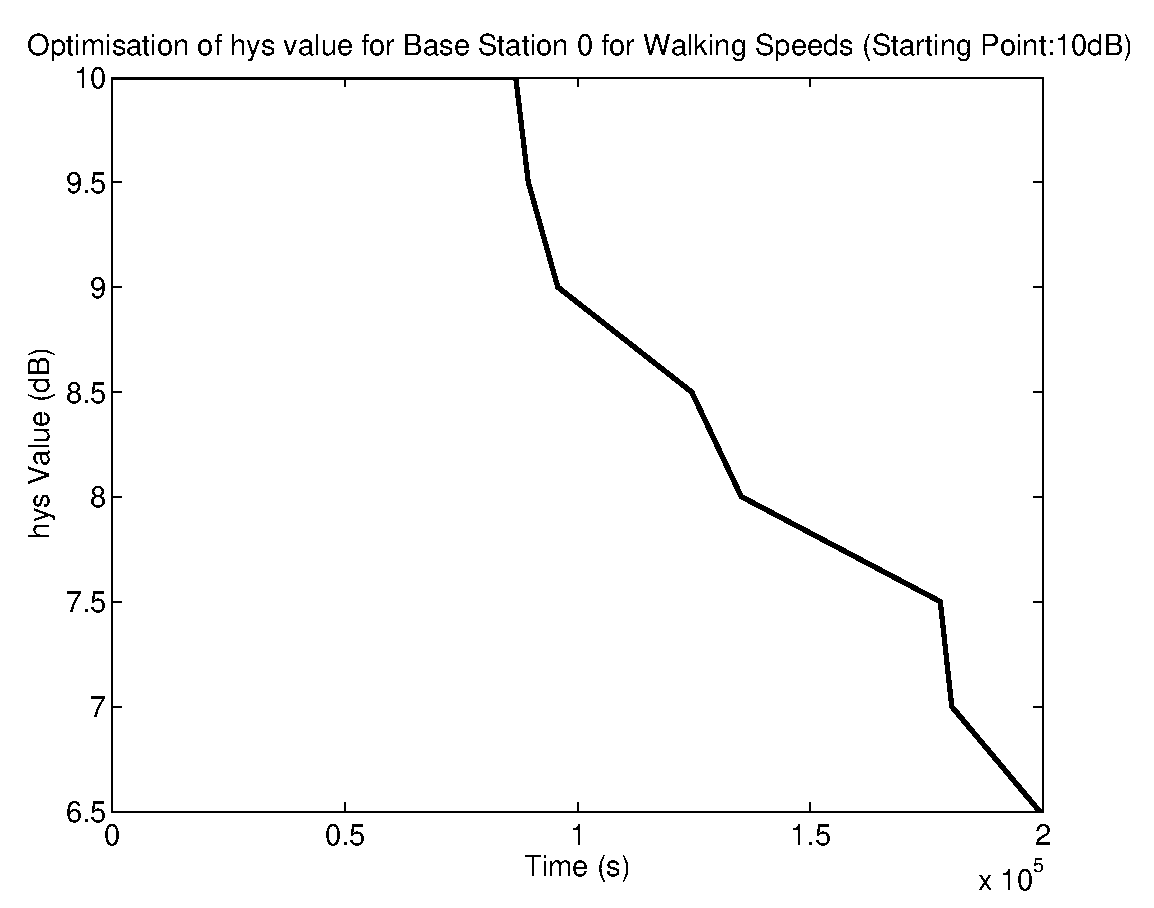
\includegraphics[width=\textwidth]{figures/graphs/walkhigh/hys0.eps}
                \caption{Changing hys Values}
        \end{subfigure}
        \caption{Illustration of how the TTT and hys values change for Base Station 0 starting at TTT=5.12s and hys=10dB with UEs moving at walking speeds.}
\end{figure}
\begin{figure}[H]
        \centering
        \begin{subfigure}[b]{0.49\textwidth}
                \includegraphics[width=\textwidth]{figures/graphs/walkhigh/TTT1.eps}
                \caption{Changing TTT Values}
        \end{subfigure}%
        ~ %add desired spacing between images, e. g. ~, \quad, \qquad etc.
          %(or a blank line to force the subfigure onto a new line)
        \begin{subfigure}[b]{0.49\textwidth}
                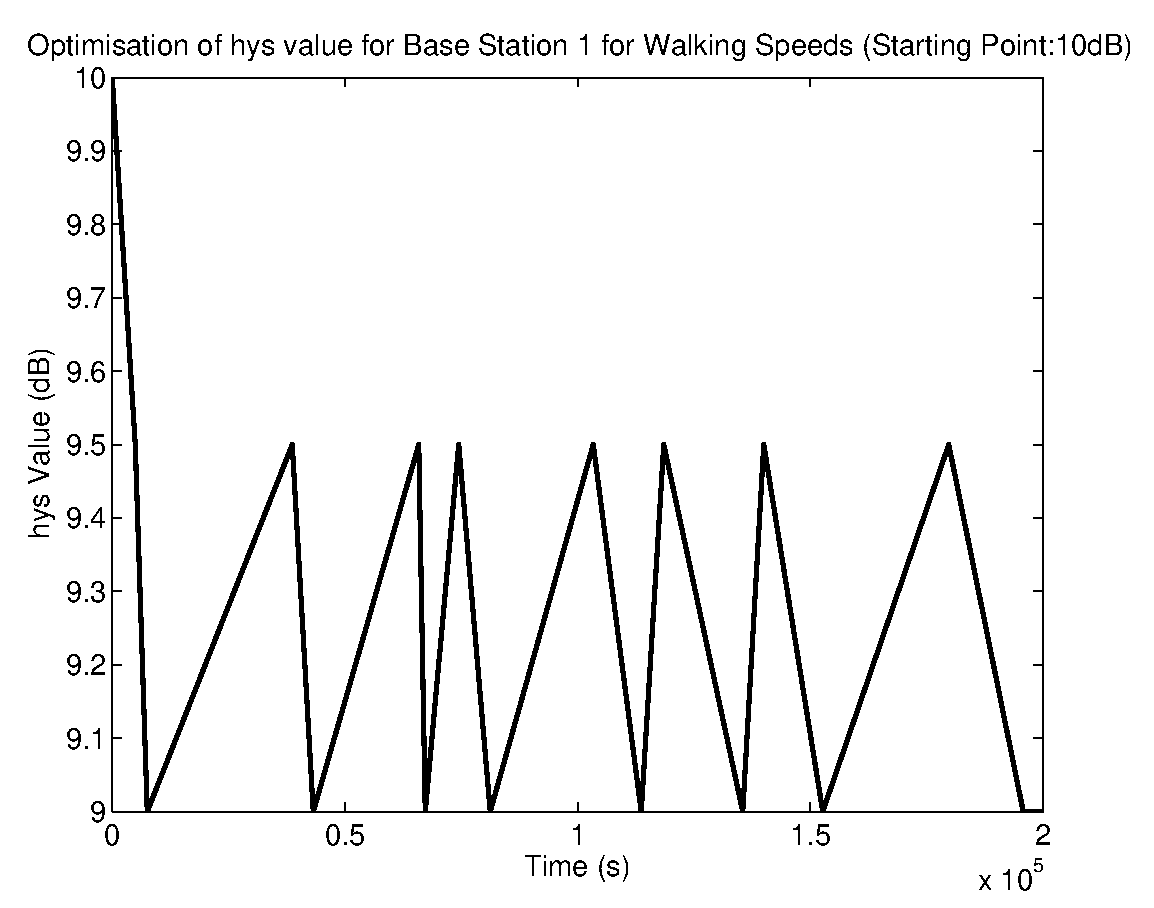
\includegraphics[width=\textwidth]{figures/graphs/walkhigh/hys1.eps}
                \caption{Changing hys Values}
        \end{subfigure}
        \caption{Illustration of how the TTT and hys values change for Base Station 1 starting at TTT=5.12s and hys=10dB with UEs moving at walking speeds.}
\end{figure}
\begin{figure}[H]
        \centering
        \begin{subfigure}[b]{0.49\textwidth}
                \includegraphics[width=\textwidth]{figures/graphs/walkhigh/TTT2.eps}
                \caption{Changing TTT Values}
        \end{subfigure}%
        ~ %add desired spacing between images, e. g. ~, \quad, \qquad etc.
          %(or a blank line to force the subfigure onto a new line)
        \begin{subfigure}[b]{0.49\textwidth}
                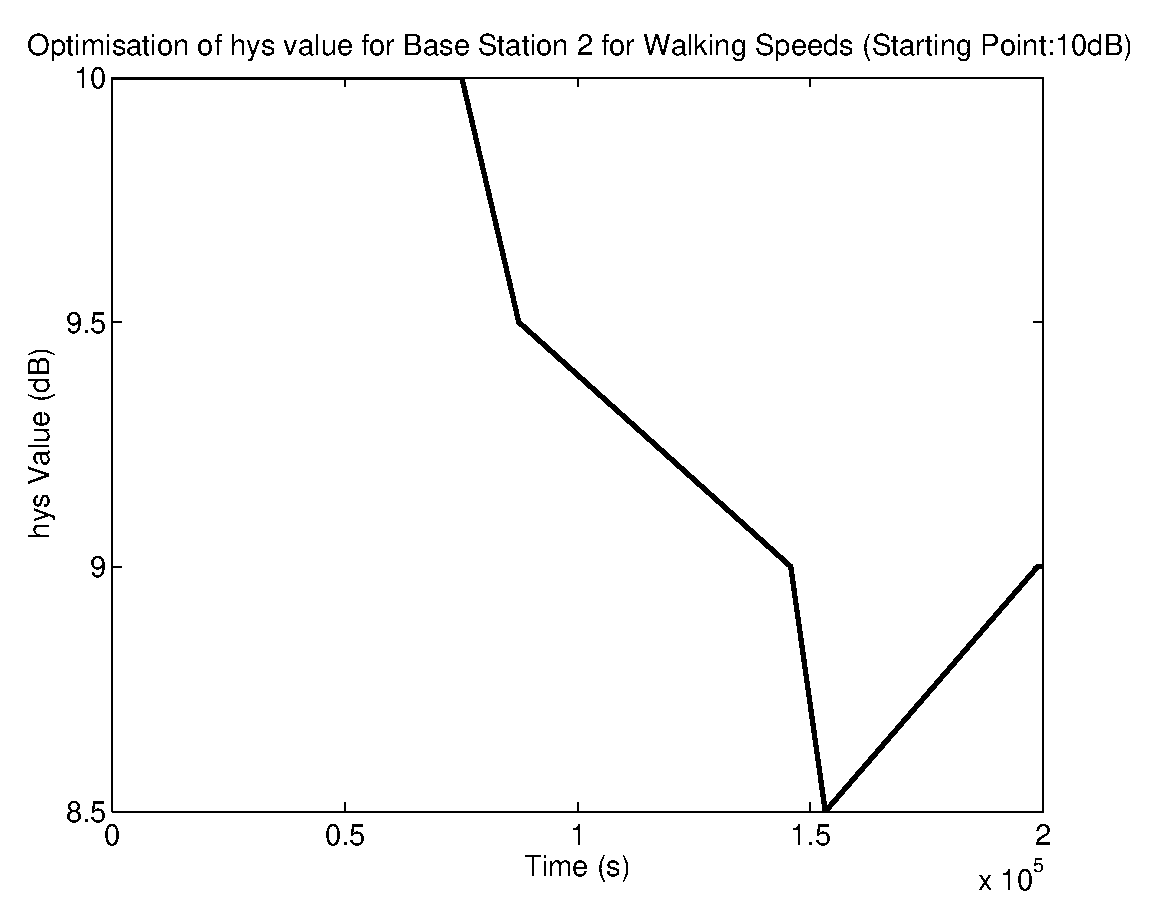
\includegraphics[width=\textwidth]{figures/graphs/walkhigh/hys2.eps}
                \caption{Changing hys Values}
        \end{subfigure}
        \caption{Illustration of how the TTT and hys values change for Base Station 2 starting at TTT=5.12s and hys=10dB with UEs moving at walking speeds.}
\end{figure}
\begin{figure}[H]
        \centering
        \begin{subfigure}[b]{0.49\textwidth}
                \includegraphics[width=\textwidth]{figures/graphs/walkhigh/TTT3.eps}
                \caption{Changing TTT Values}
        \end{subfigure}%
        ~ %add desired spacing between images, e. g. ~, \quad, \qquad etc.
          %(or a blank line to force the subfigure onto a new line)
        \begin{subfigure}[b]{0.49\textwidth}
                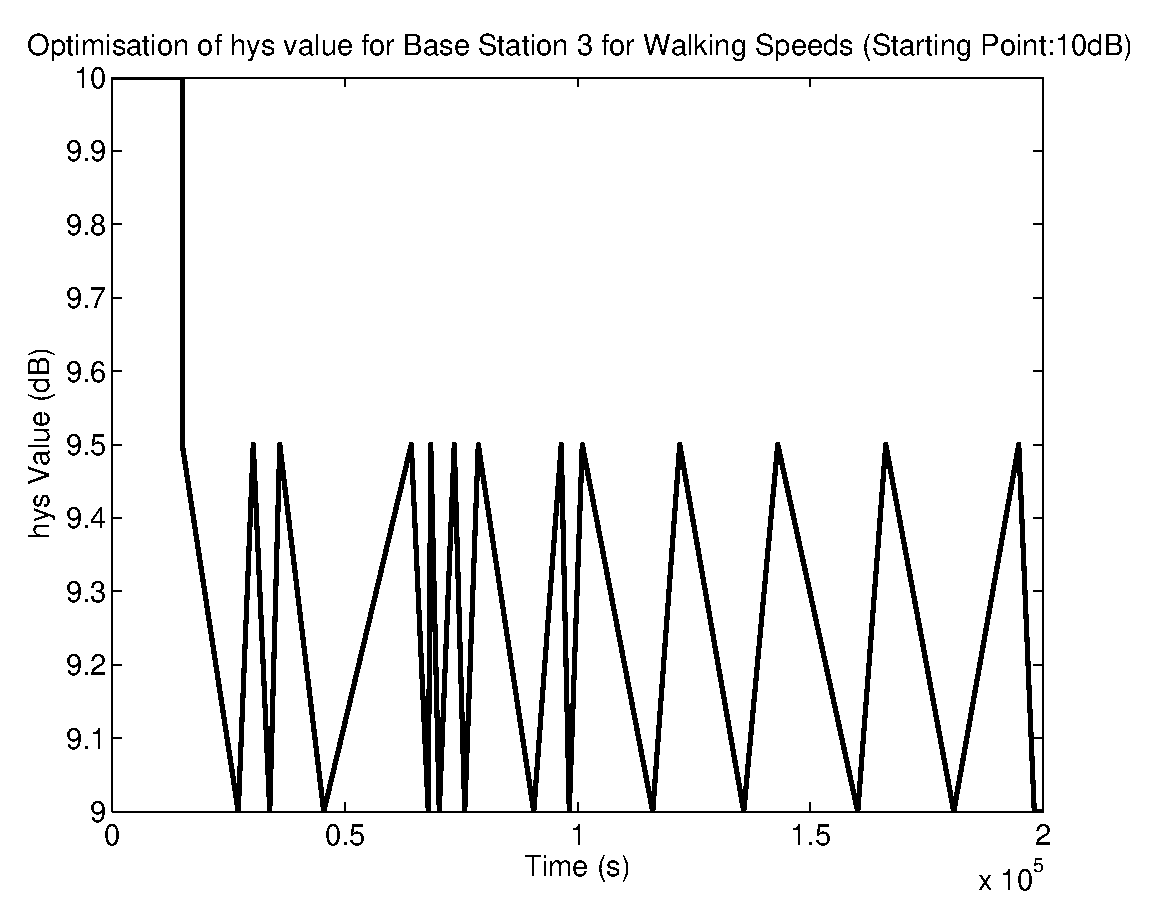
\includegraphics[width=\textwidth]{figures/graphs/walkhigh/hys3.eps}
                \caption{Changing hys Values}
        \end{subfigure}
        \caption{Illustration of how the TTT and hys values change for Base Station 3 starting at TTT=5.12s and hys=10dB with UEs moving at walking speeds.}
\end{figure}
\begin{figure}[H]
        \centering
        \begin{subfigure}[b]{0.49\textwidth}
                \includegraphics[width=\textwidth]{figures/graphs/walkhigh/TTT4.eps}
                \caption{Changing TTT Values}
        \end{subfigure}%
        ~ %add desired spacing between images, e. g. ~, \quad, \qquad etc.
          %(or a blank line to force the subfigure onto a new line)
        \begin{subfigure}[b]{0.49\textwidth}
                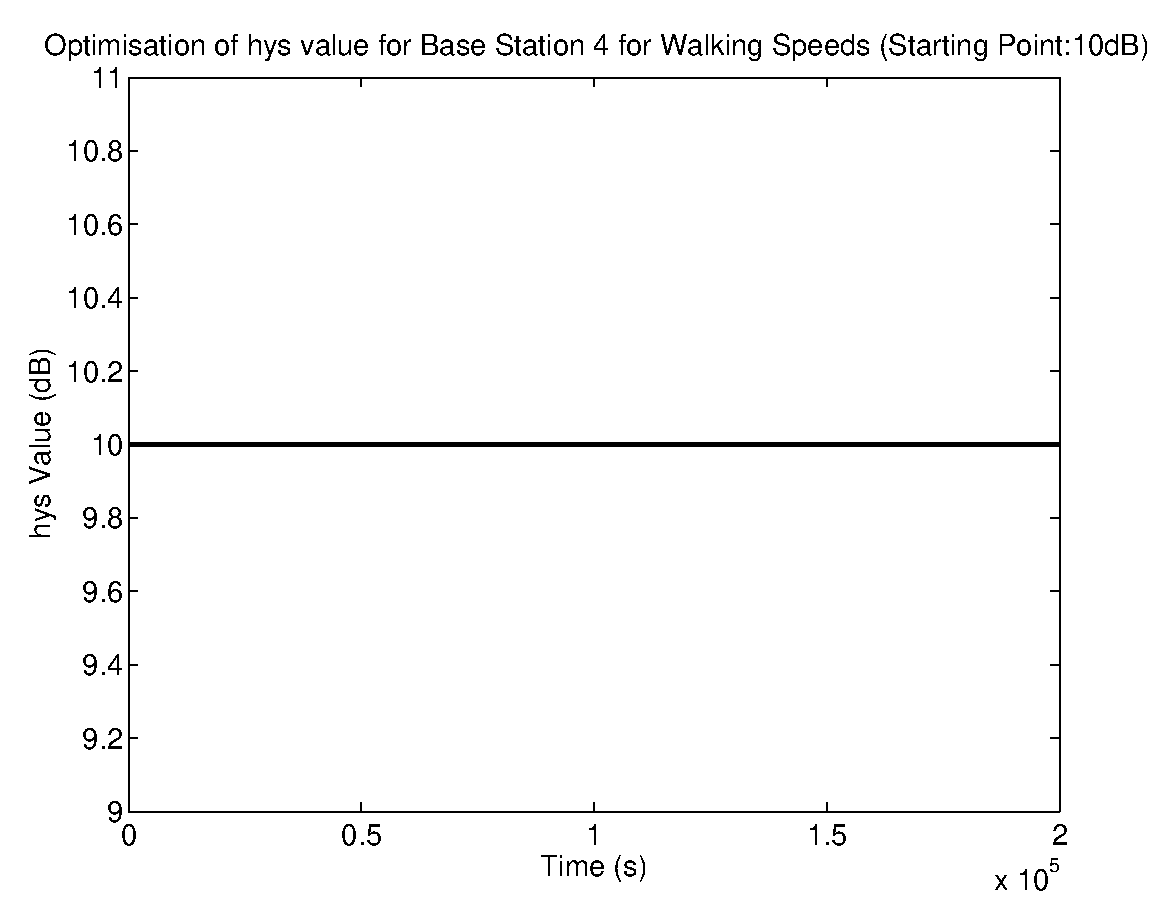
\includegraphics[width=\textwidth]{figures/graphs/walkhigh/hys4.eps}
                \caption{Changing hys Values}
        \end{subfigure}
        \caption{Illustration of how the TTT and hys values change for Base Station 4 starting at TTT=5.12s and hys=10dB with UEs moving at walking speeds.}
\end{figure}
\begin{figure}[H]
        \centering
        \begin{subfigure}[b]{0.49\textwidth}
                \includegraphics[width=\textwidth]{figures/graphs/walkhigh/TTT5.eps}
                \caption{Changing TTT Values}
        \end{subfigure}%
        ~ %add desired spacing between images, e. g. ~, \quad, \qquad etc.
          %(or a blank line to force the subfigure onto a new line)
        \begin{subfigure}[b]{0.49\textwidth}
                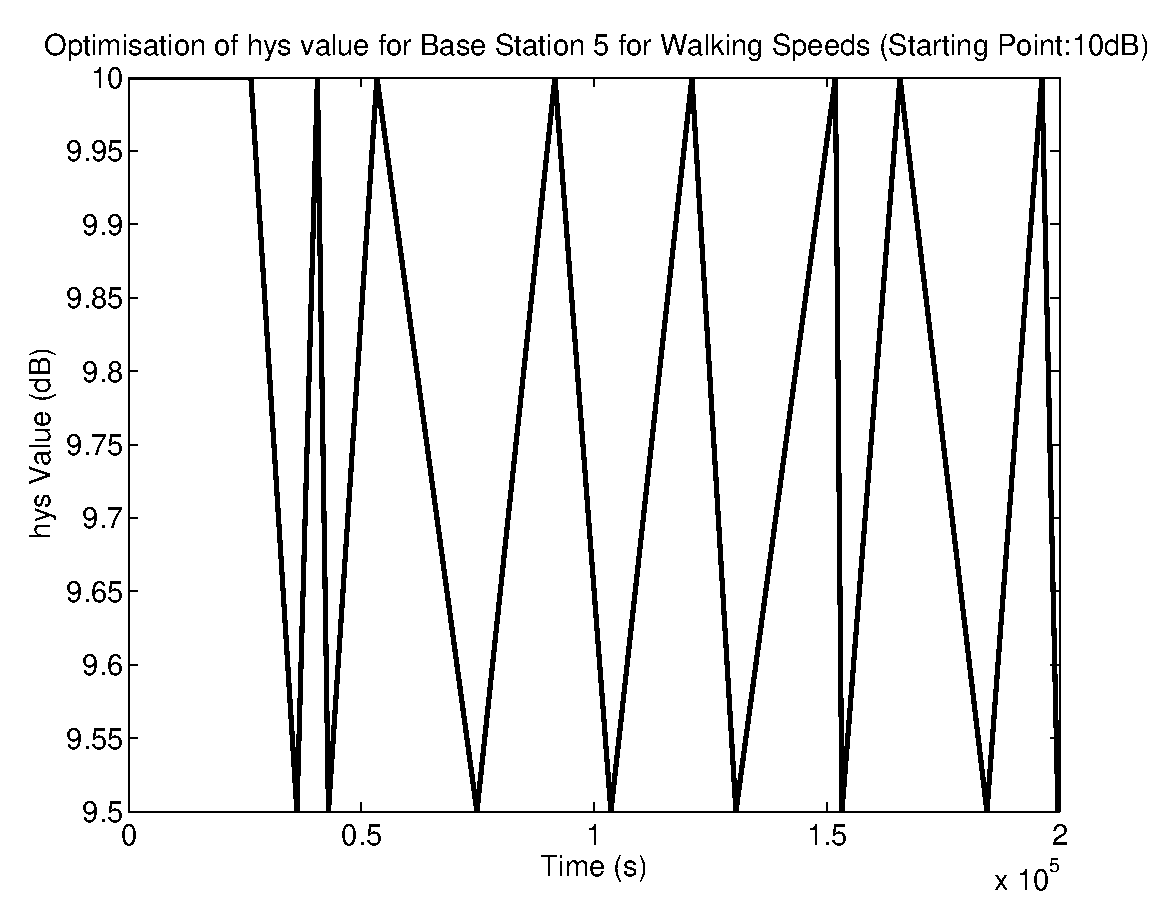
\includegraphics[width=\textwidth]{figures/graphs/walkhigh/hys5.eps}
                \caption{Changing hys Values}
        \end{subfigure}
        \caption{Illustration of how the TTT and hys values change for Base Station 5 starting at TTT=5.12s and hys=10dB with UEs moving at walking speeds.}
\end{figure}
\begin{figure}[H]
        \centering
        \begin{subfigure}[b]{0.49\textwidth}
                \includegraphics[width=\textwidth]{figures/graphs/walkhigh/TTT6.eps}
                \caption{Changing TTT Values}
        \end{subfigure}%
        ~ %add desired spacing between images, e. g. ~, \quad, \qquad etc.
          %(or a blank line to force the subfigure onto a new line)
        \begin{subfigure}[b]{0.49\textwidth}
                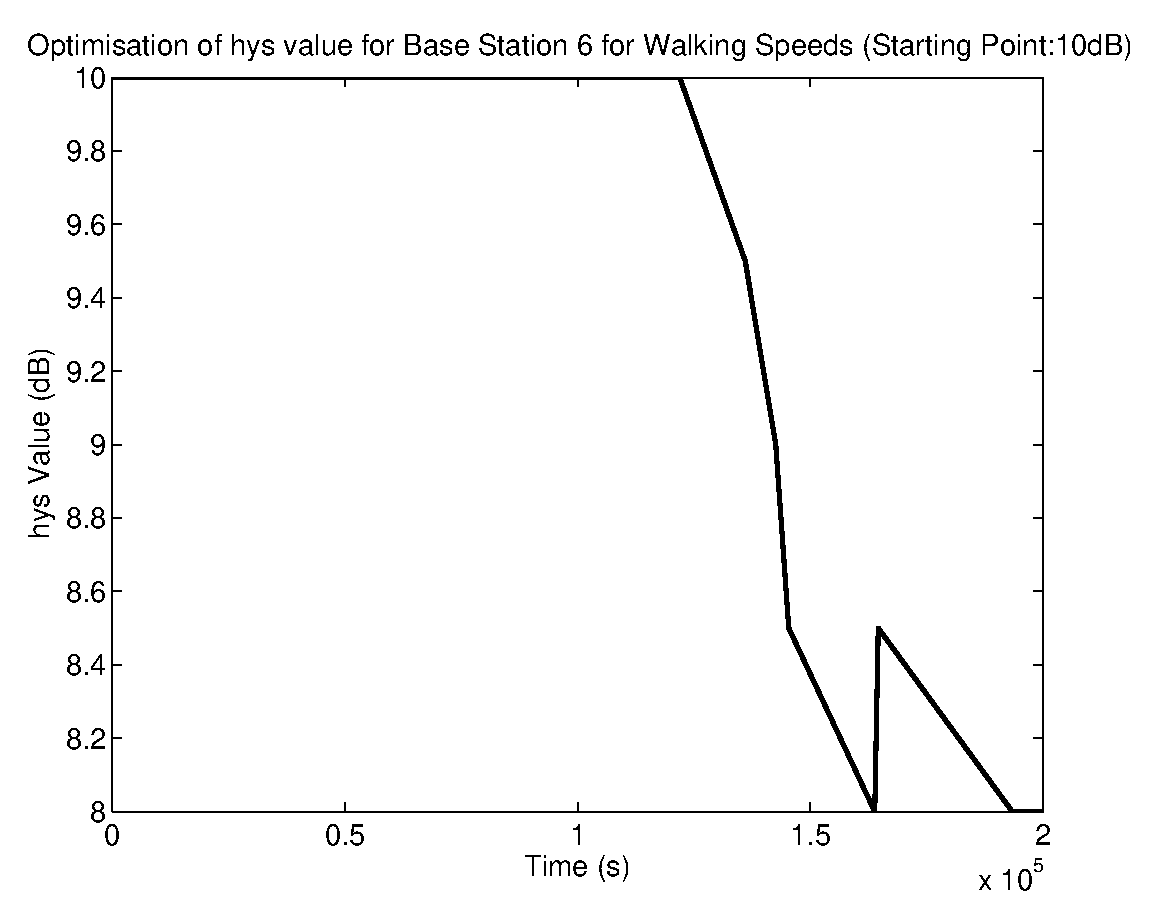
\includegraphics[width=\textwidth]{figures/graphs/walkhigh/hys6.eps}
                \caption{Changing hys Values}
        \end{subfigure}
        \caption{Illustration of how the TTT and hys values change for Base Station 6 starting at TTT=5.12s and hys=10dB with UEs moving at walking speeds.}
\end{figure}
\begin{figure}[H]
        \centering
        \begin{subfigure}[b]{0.49\textwidth}
                \includegraphics[width=\textwidth]{figures/graphs/walkhigh/TTT7.eps}
                \caption{Changing TTT Values}
        \end{subfigure}%
        ~ %add desired spacing between images, e. g. ~, \quad, \qquad etc.
          %(or a blank line to force the subfigure onto a new line)
        \begin{subfigure}[b]{0.49\textwidth}
                \includegraphics[width=\textwidth]{figures/graphs/walkhigh/hys7.eps}
                \caption{Changing hys Values}
        \end{subfigure}
        \caption{Illustration of how the TTT and hys values change for Base Station 7 starting at TTT=5.12s and hys=10dB with UEs moving at walking speeds.}
\end{figure}
\begin{figure}[H]
        \centering
        \begin{subfigure}[b]{0.49\textwidth}
                \includegraphics[width=\textwidth]{figures/graphs/walkhigh/TTT8.eps}
                \caption{Changing TTT Values}
        \end{subfigure}%
        ~ %add desired spacing between images, e. g. ~, \quad, \qquad etc.
          %(or a blank line to force the subfigure onto a new line)
        \begin{subfigure}[b]{0.49\textwidth}
                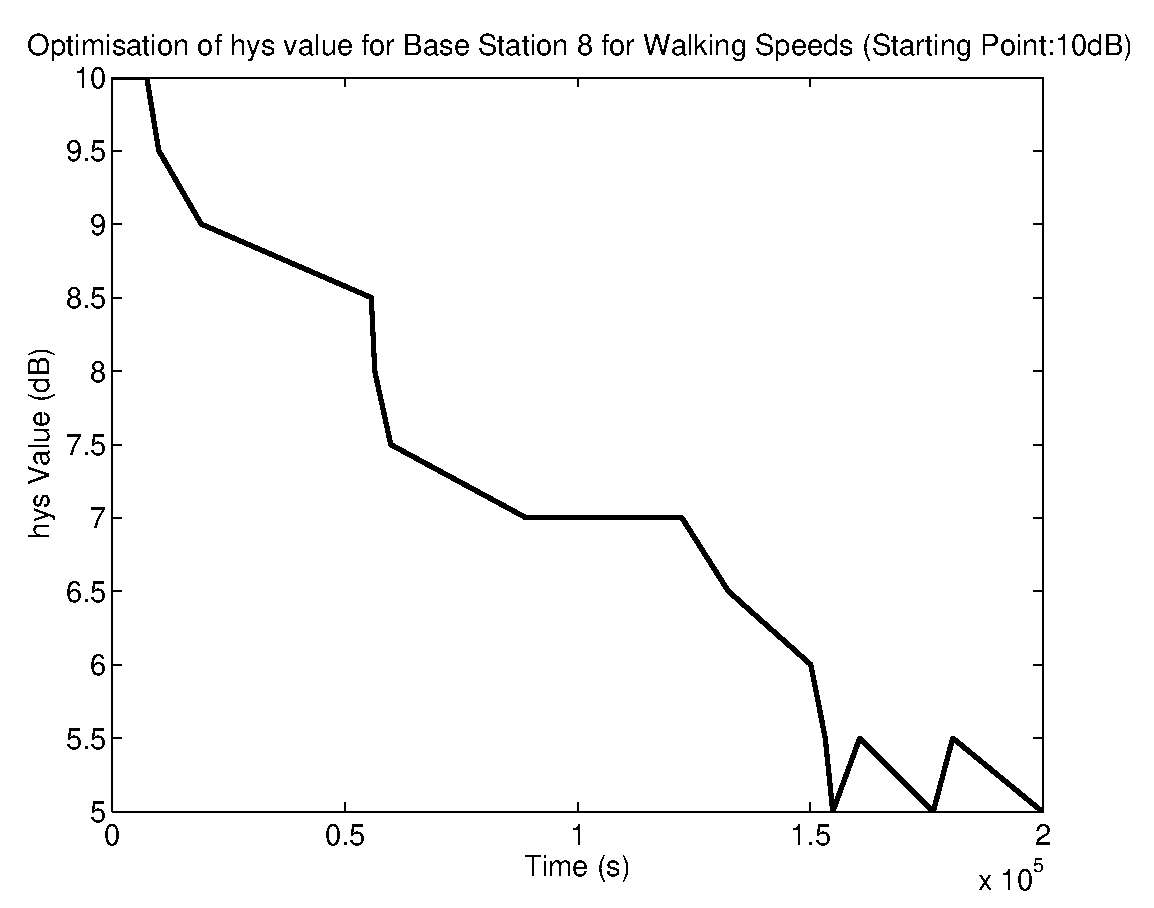
\includegraphics[width=\textwidth]{figures/graphs/walkhigh/hys8.eps}
                \caption{Changing hys Values}
        \end{subfigure}
        \caption{Illustration of how the TTT and hys values change for Base Station 8 starting at TTT=5.12s and hys=10dB with UEs moving at walking speeds.}
\end{figure}
\subsection{Middle Starting Values}\label{ap:walk_mid}
\begin{figure}[H]
        \centering
        \begin{subfigure}[b]{0.49\textwidth}
                \includegraphics[width=\textwidth]{figures/graphs/walkmid/TTT0.eps}
                \caption{Changing TTT Values}
        \end{subfigure}%
        ~ %add desired spacing between images, e. g. ~, \quad, \qquad etc.
          %(or a blank line to force the subfigure onto a new line)
        \begin{subfigure}[b]{0.49\textwidth}
                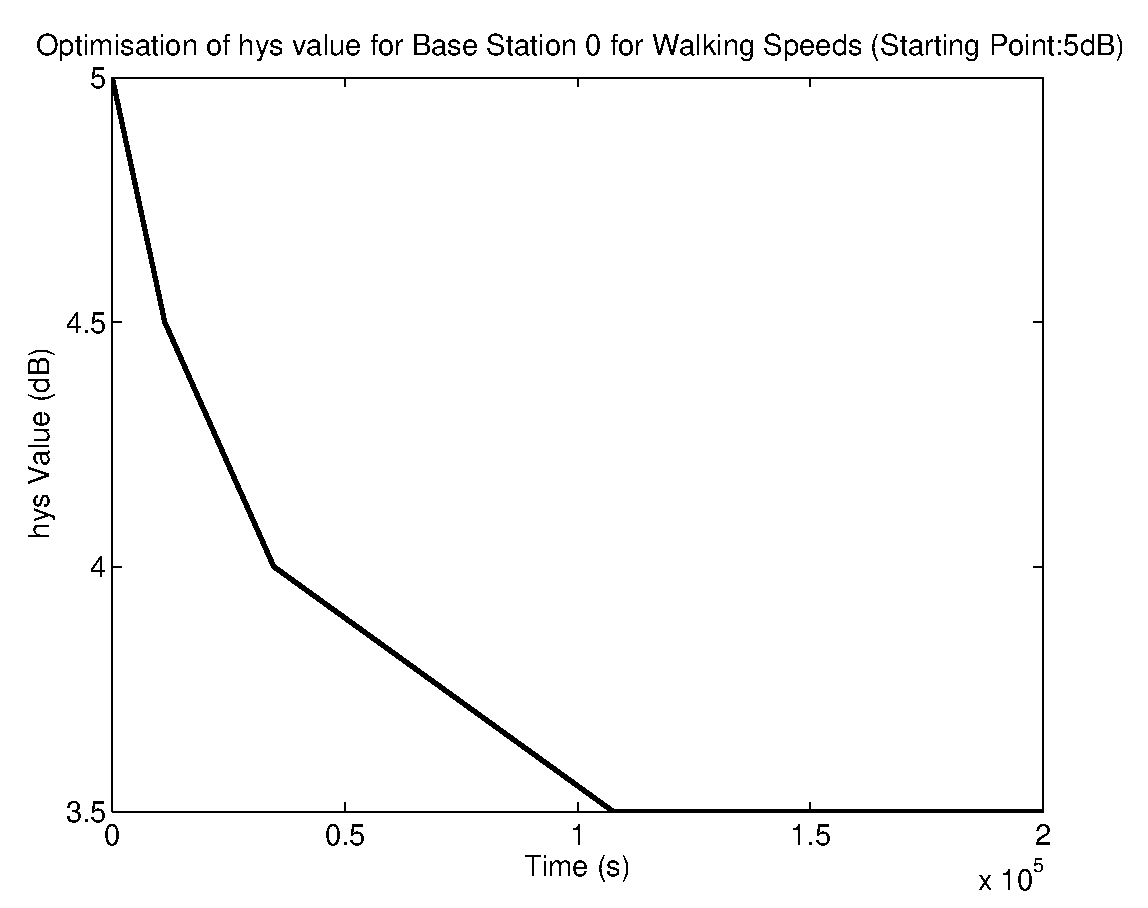
\includegraphics[width=\textwidth]{figures/graphs/walkmid/hys0.eps}
                \caption{Changing hys Values}
        \end{subfigure}
        \caption{Illustration of how the TTT and hys values change for Base Station 0 starting at TTT=0.256s and hys=5dB with UEs moving at walking speeds.}
\end{figure}
\begin{figure}[H]
        \centering
        \begin{subfigure}[b]{0.49\textwidth}
                \includegraphics[width=\textwidth]{figures/graphs/walkmid/TTT1.eps}
                \caption{Changing TTT Values}
        \end{subfigure}%
        ~ %add desired spacing between images, e. g. ~, \quad, \qquad etc.
          %(or a blank line to force the subfigure onto a new line)
        \begin{subfigure}[b]{0.49\textwidth}
                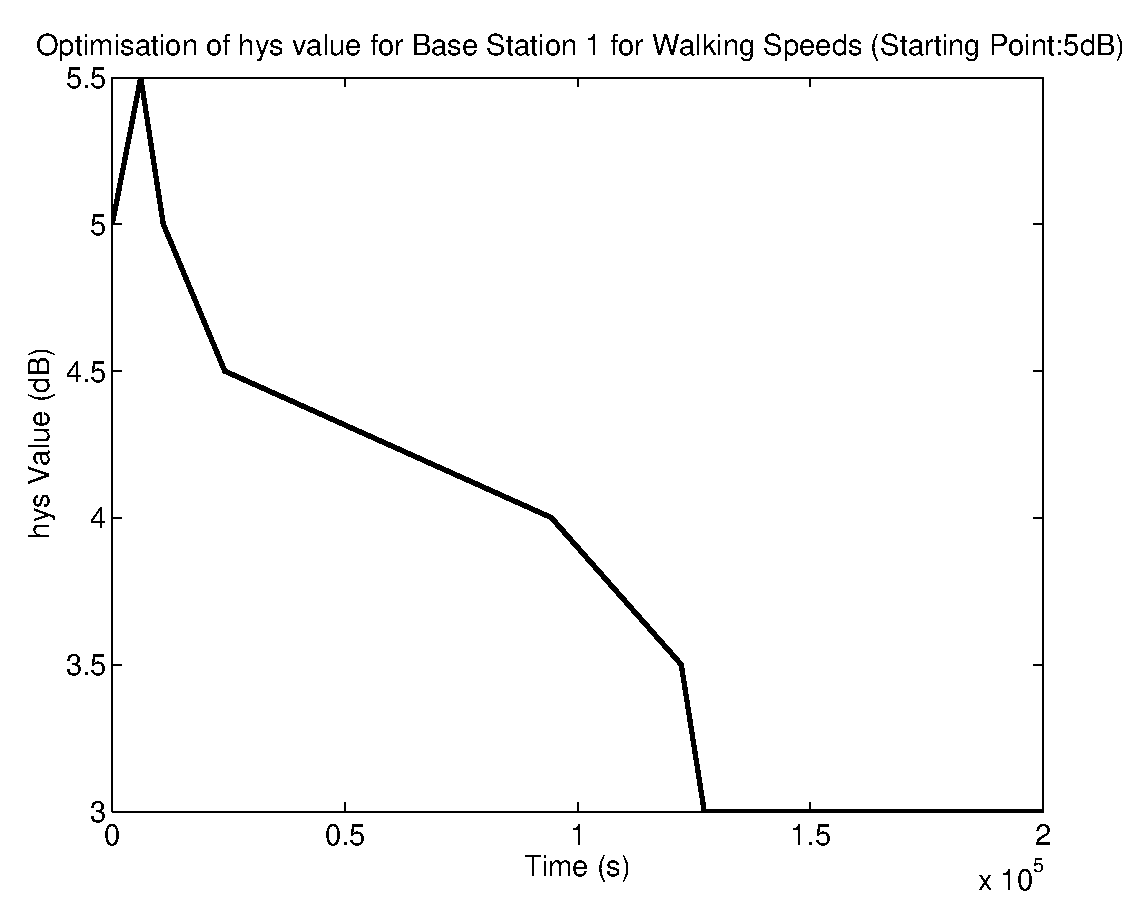
\includegraphics[width=\textwidth]{figures/graphs/walkmid/hys1.eps}
                \caption{Changing hys Values}
        \end{subfigure}
        \caption{Illustration of how the TTT and hys values change for Base Station 1 starting at TTT=0.256s and hys=5dB with UEs moving at walking speeds.}
\end{figure}
\begin{figure}[H]
        \centering
        \begin{subfigure}[b]{0.49\textwidth}
                \includegraphics[width=\textwidth]{figures/graphs/walkmid/TTT2.eps}
                \caption{Changing TTT Values}
        \end{subfigure}%
        ~ %add desired spacing between images, e. g. ~, \quad, \qquad etc.
          %(or a blank line to force the subfigure onto a new line)
        \begin{subfigure}[b]{0.49\textwidth}
                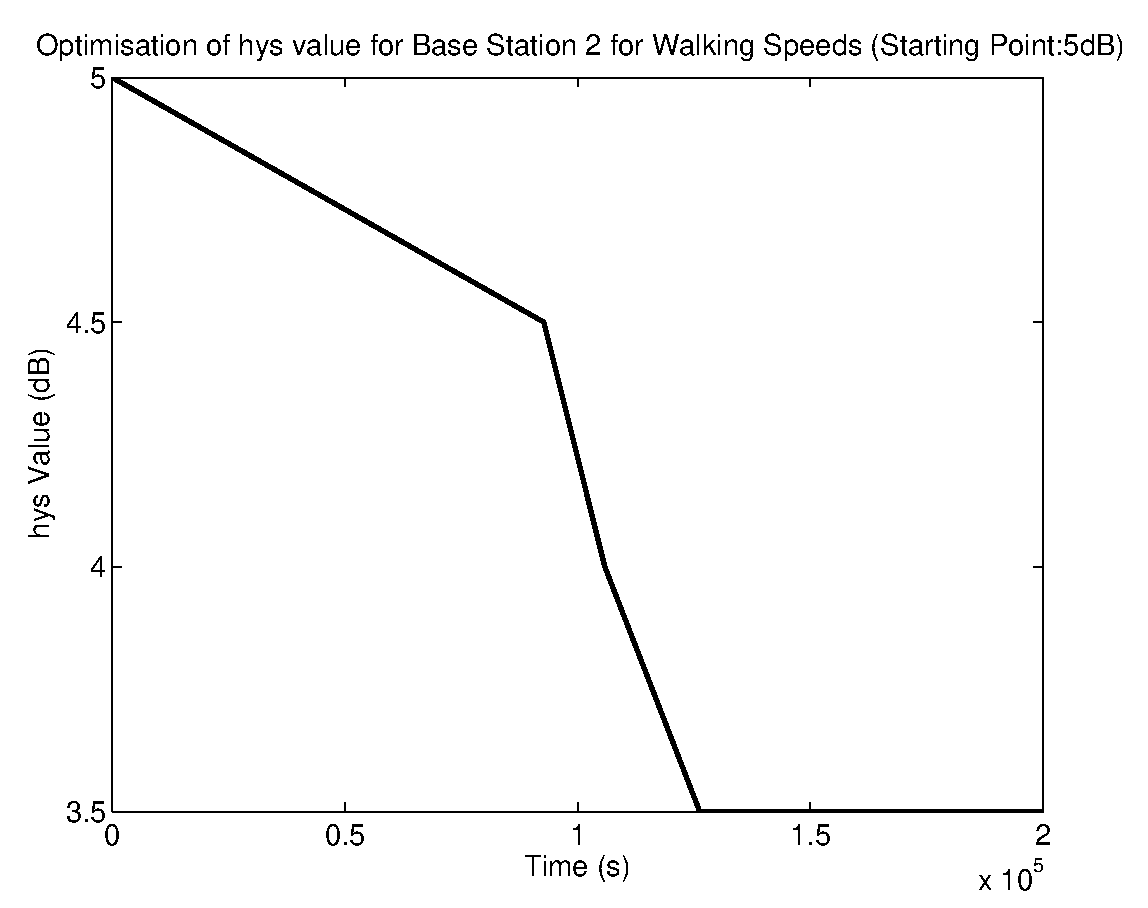
\includegraphics[width=\textwidth]{figures/graphs/walkmid/hys2.eps}
                \caption{Changing hys Values}
        \end{subfigure}
        \caption{Illustration of how the TTT and hys values change for Base Station 2 starting at TTT=0.256s and hys=5dB with UEs moving at walking speeds.}
\end{figure}
\begin{figure}[H]
        \centering
        \begin{subfigure}[b]{0.49\textwidth}
                \includegraphics[width=\textwidth]{figures/graphs/walkmid/TTT3.eps}
                \caption{Changing TTT Values}
        \end{subfigure}%
        ~ %add desired spacing between images, e. g. ~, \quad, \qquad etc.
          %(or a blank line to force the subfigure onto a new line)
        \begin{subfigure}[b]{0.49\textwidth}
                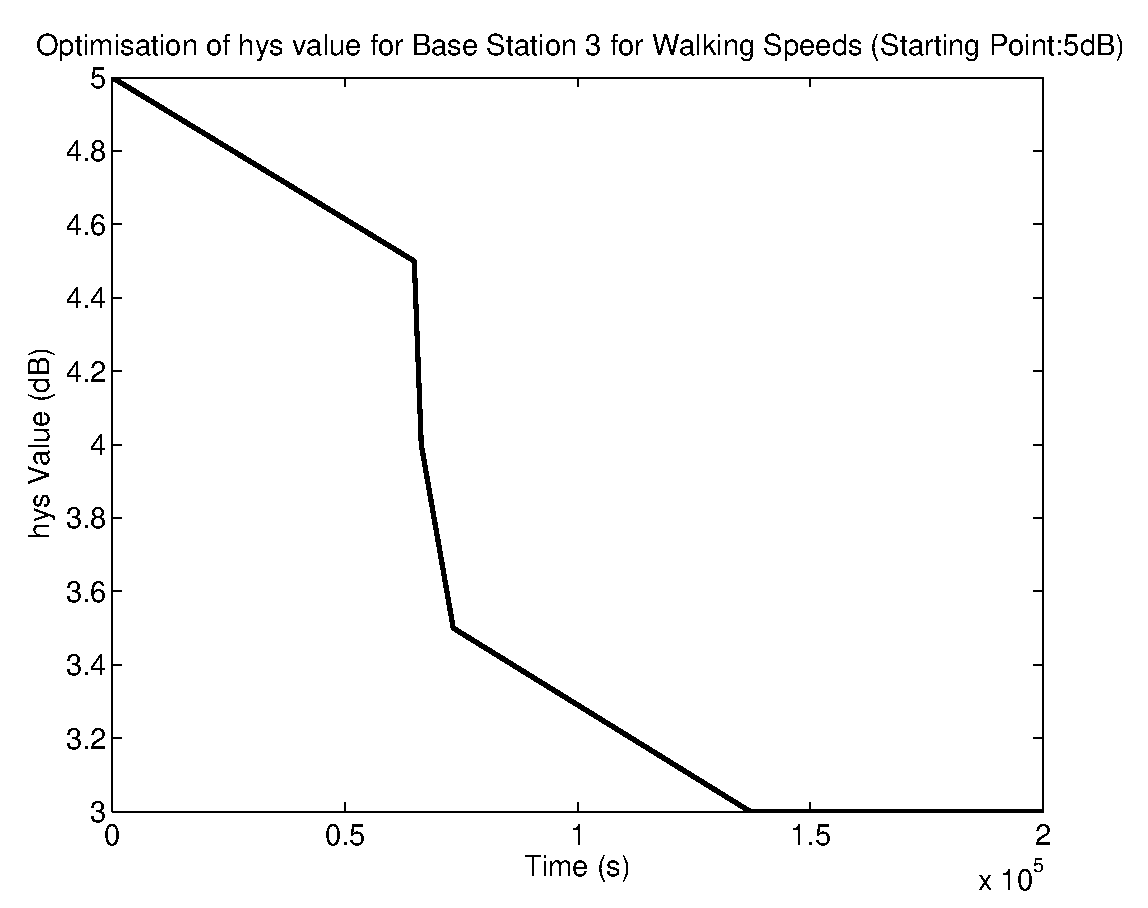
\includegraphics[width=\textwidth]{figures/graphs/walkmid/hys3.eps}
                \caption{Changing hys Values}
        \end{subfigure}
        \caption{Illustration of how the TTT and hys values change for Base Station 3 starting at TTT=0.256s and hys=5dB with UEs moving at walking speeds.}
\end{figure}
\begin{figure}[H]
        \centering
        \begin{subfigure}[b]{0.49\textwidth}
                \includegraphics[width=\textwidth]{figures/graphs/walkmid/TTT4.eps}
                \caption{Changing TTT Values}
        \end{subfigure}%
        ~ %add desired spacing between images, e. g. ~, \quad, \qquad etc.
          %(or a blank line to force the subfigure onto a new line)
        \begin{subfigure}[b]{0.49\textwidth}
                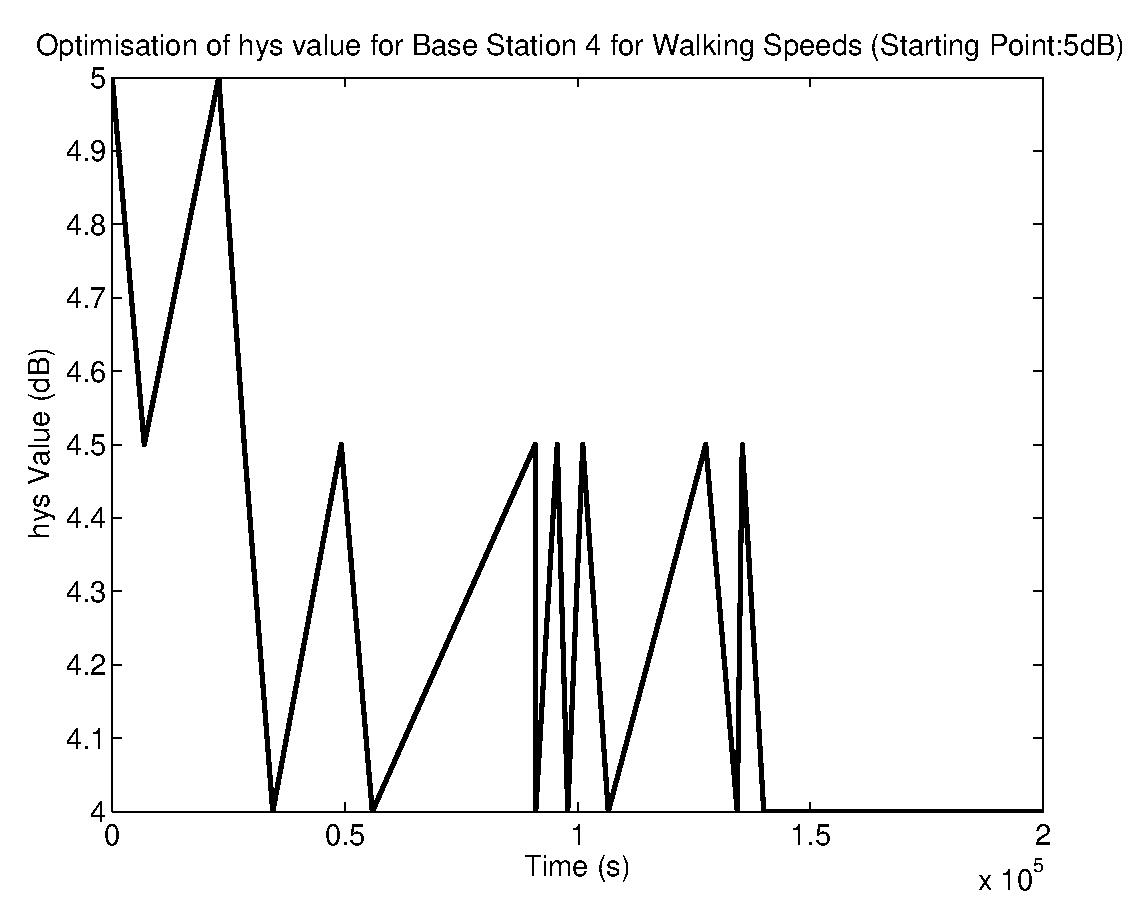
\includegraphics[width=\textwidth]{figures/graphs/walkmid/hys4.eps}
                \caption{Changing hys Values}
        \end{subfigure}
        \caption{Illustration of how the TTT and hys values change for Base Station 4 starting at TTT=0.256s and hys=5dB with UEs moving at walking speeds.}
\end{figure}
\begin{figure}[H]
        \centering
        \begin{subfigure}[b]{0.49\textwidth}
                \includegraphics[width=\textwidth]{figures/graphs/walkmid/TTT5.eps}
                \caption{Changing TTT Values}
        \end{subfigure}%
        ~ %add desired spacing between images, e. g. ~, \quad, \qquad etc.
          %(or a blank line to force the subfigure onto a new line)
        \begin{subfigure}[b]{0.49\textwidth}
                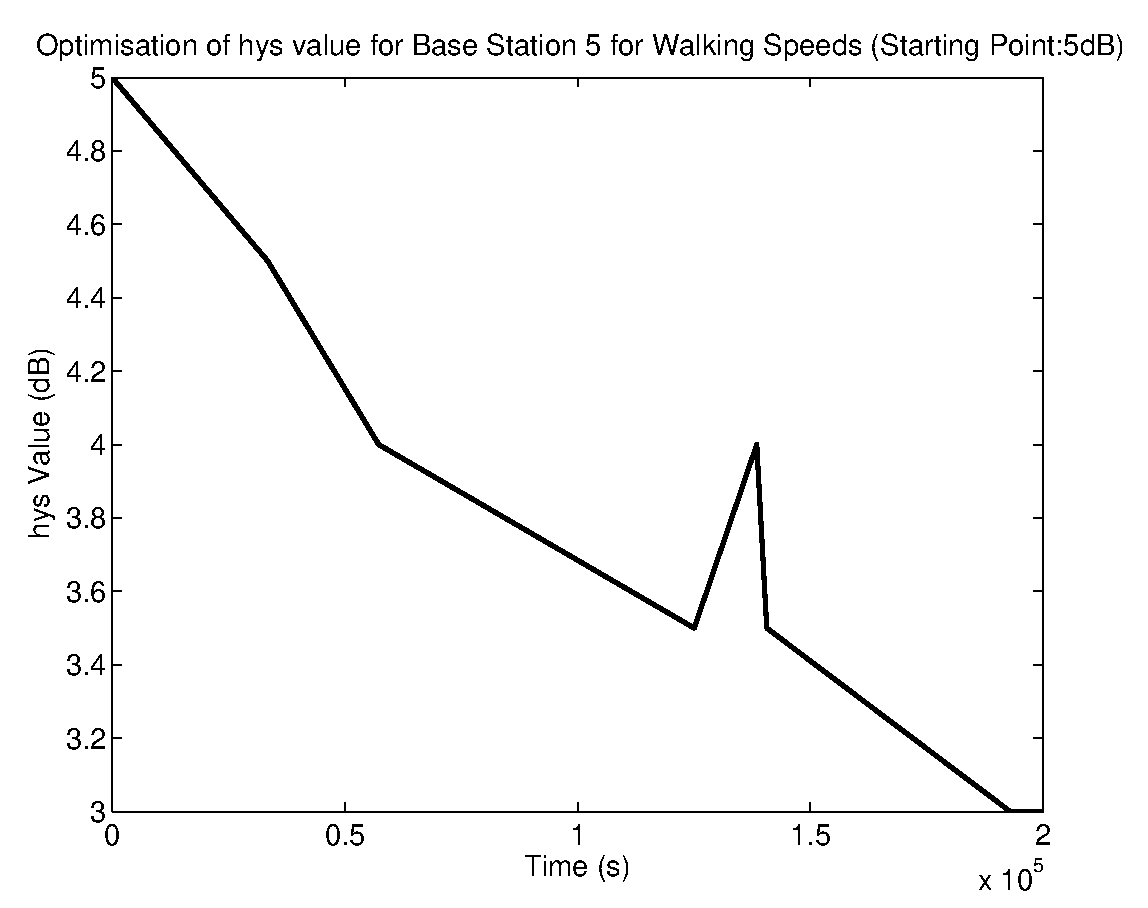
\includegraphics[width=\textwidth]{figures/graphs/walkmid/hys5.eps}
                \caption{Changing hys Values}
        \end{subfigure}
        \caption{Illustration of how the TTT and hys values change for Base Station 5 starting at TTT=0.256s and hys=5dB with UEs moving at walking speeds.}
\end{figure}
\begin{figure}[H]
        \centering
        \begin{subfigure}[b]{0.49\textwidth}
                \includegraphics[width=\textwidth]{figures/graphs/walkmid/TTT6.eps}
                \caption{Changing TTT Values}
        \end{subfigure}%
        ~ %add desired spacing between images, e. g. ~, \quad, \qquad etc.
          %(or a blank line to force the subfigure onto a new line)
        \begin{subfigure}[b]{0.49\textwidth}
                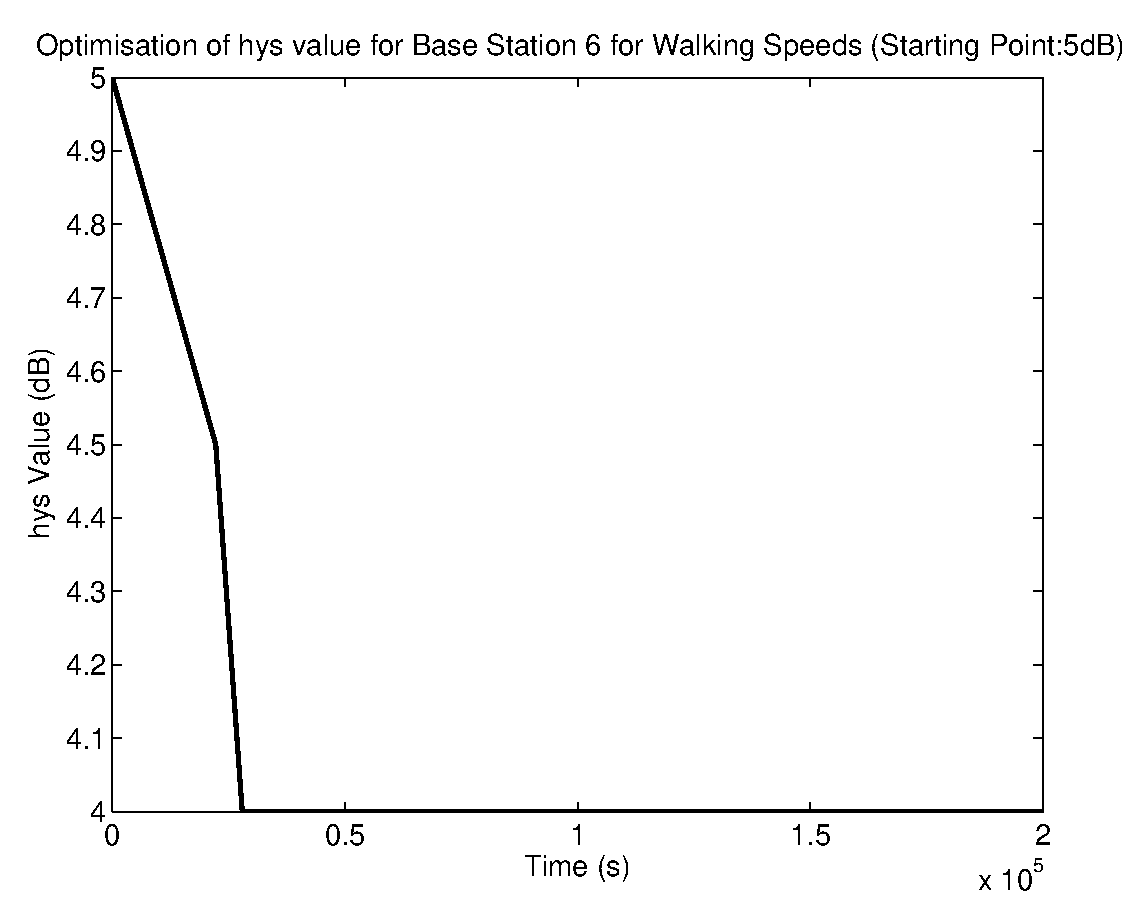
\includegraphics[width=\textwidth]{figures/graphs/walkmid/hys6.eps}
                \caption{Changing hys Values}
        \end{subfigure}
        \caption{Illustration of how the TTT and hys values change for Base Station 6 starting at TTT=0.256s and hys=5dB with UEs moving at walking speeds.}
\end{figure}
\begin{figure}[H]
        \centering
        \begin{subfigure}[b]{0.49\textwidth}
                \includegraphics[width=\textwidth]{figures/graphs/walkmid/TTT7.eps}
                \caption{Changing TTT Values}
        \end{subfigure}%
        ~ %add desired spacing between images, e. g. ~, \quad, \qquad etc.
          %(or a blank line to force the subfigure onto a new line)
        \begin{subfigure}[b]{0.49\textwidth}
                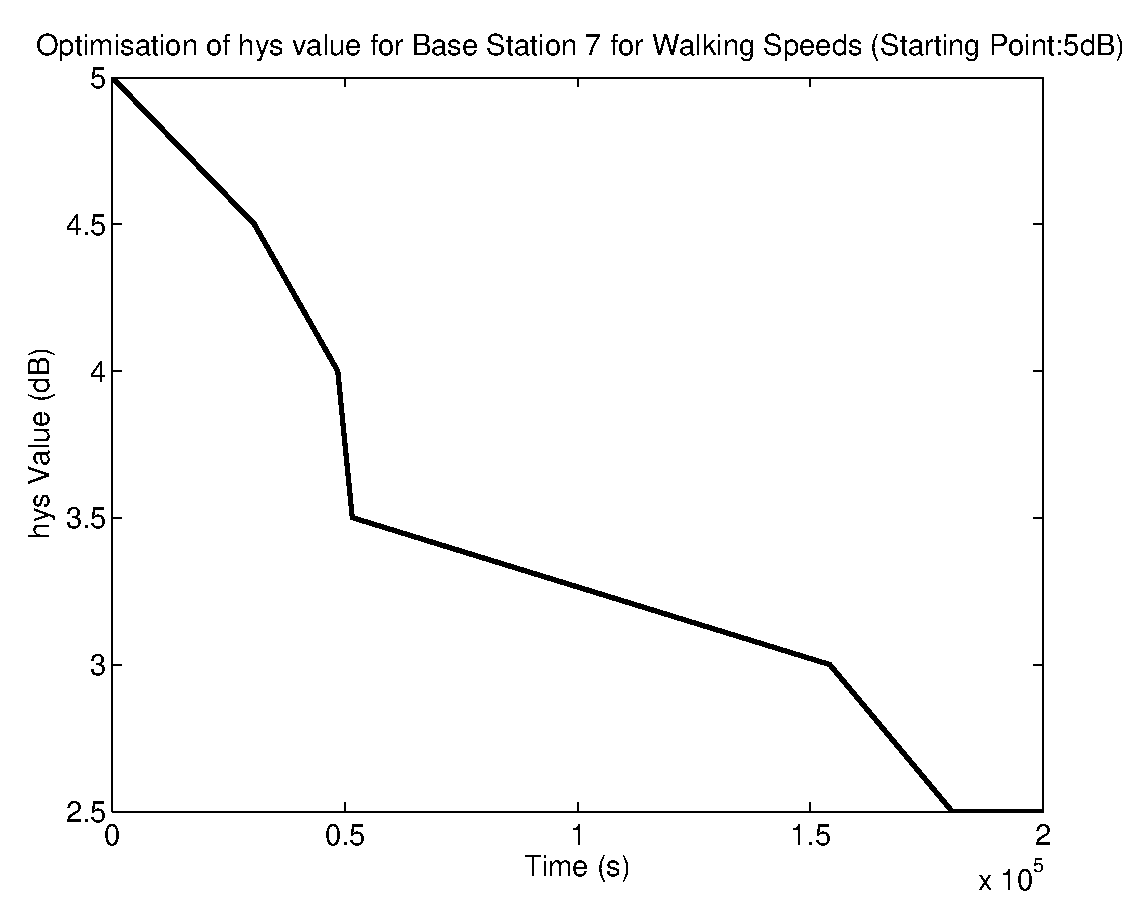
\includegraphics[width=\textwidth]{figures/graphs/walkmid/hys7.eps}
                \caption{Changing hys Values}
        \end{subfigure}
        \caption{Illustration of how the TTT and hys values change for Base Station 7 starting at TTT=0.256s and hys=5dB with UEs moving at walking speeds.}
\end{figure}
\begin{figure}[H]
        \centering
        \begin{subfigure}[b]{0.49\textwidth}
                \includegraphics[width=\textwidth]{figures/graphs/walkmid/TTT8.eps}
                \caption{Changing TTT Values}
        \end{subfigure}%
        ~ %add desired spacing between images, e. g. ~, \quad, \qquad etc.
          %(or a blank line to force the subfigure onto a new line)
        \begin{subfigure}[b]{0.49\textwidth}
                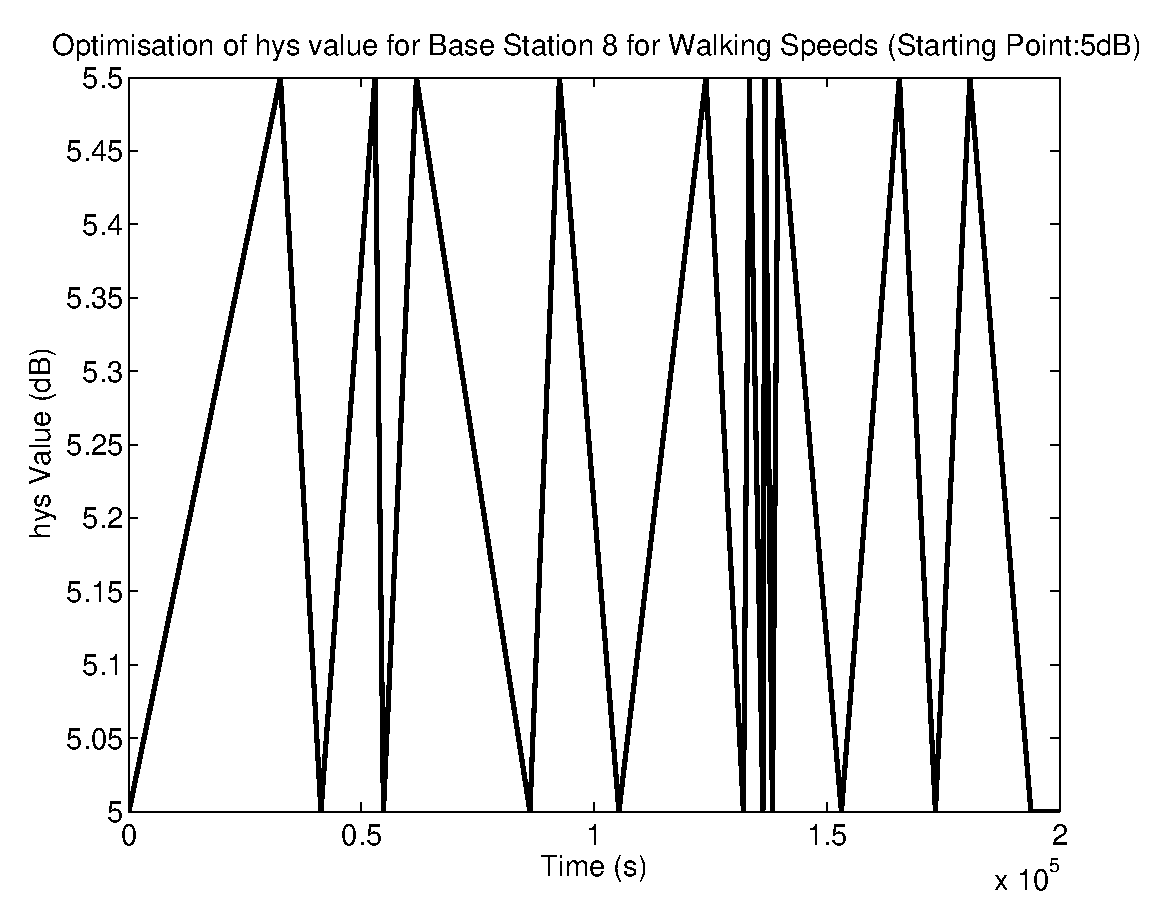
\includegraphics[width=\textwidth]{figures/graphs/walkmid/hys8.eps}
                \caption{Changing hys Values}
        \end{subfigure}
        \caption{Illustration of how the TTT and hys values change for Base Station 8 starting at TTT=0.256s and hys=5dB with UEs moving at walking speeds.}
\end{figure}
\subsection{Small Starting Values}\label{ap:walk_low}
\begin{figure}[H]
        \centering
        \begin{subfigure}[b]{0.49\textwidth}
                \includegraphics[width=\textwidth]{figures/graphs/walklow/TTT0.eps}
                \caption{Changing TTT Values}
        \end{subfigure}%
        ~ %add desired spacing between images, e. g. ~, \quad, \qquad etc.
          %(or a blank line to force the subfigure onto a new line)
        \begin{subfigure}[b]{0.49\textwidth}
                \includegraphics[width=\textwidth]{figures/graphs/walklow/hys0.eps}
                \caption{Changing hys Values}
        \end{subfigure}
        \caption{Illustration of how the TTT and hys values change for Base Station 0 starting at TTT=0s and hys=0dB with UEs moving at walking speeds.}
\end{figure}
\begin{figure}[H]
        \centering
        \begin{subfigure}[b]{0.49\textwidth}
                \includegraphics[width=\textwidth]{figures/graphs/walklow/TTT1.eps}
                \caption{Changing TTT Values}
        \end{subfigure}%
        ~ %add desired spacing between images, e. g. ~, \quad, \qquad etc.
          %(or a blank line to force the subfigure onto a new line)
        \begin{subfigure}[b]{0.49\textwidth}
                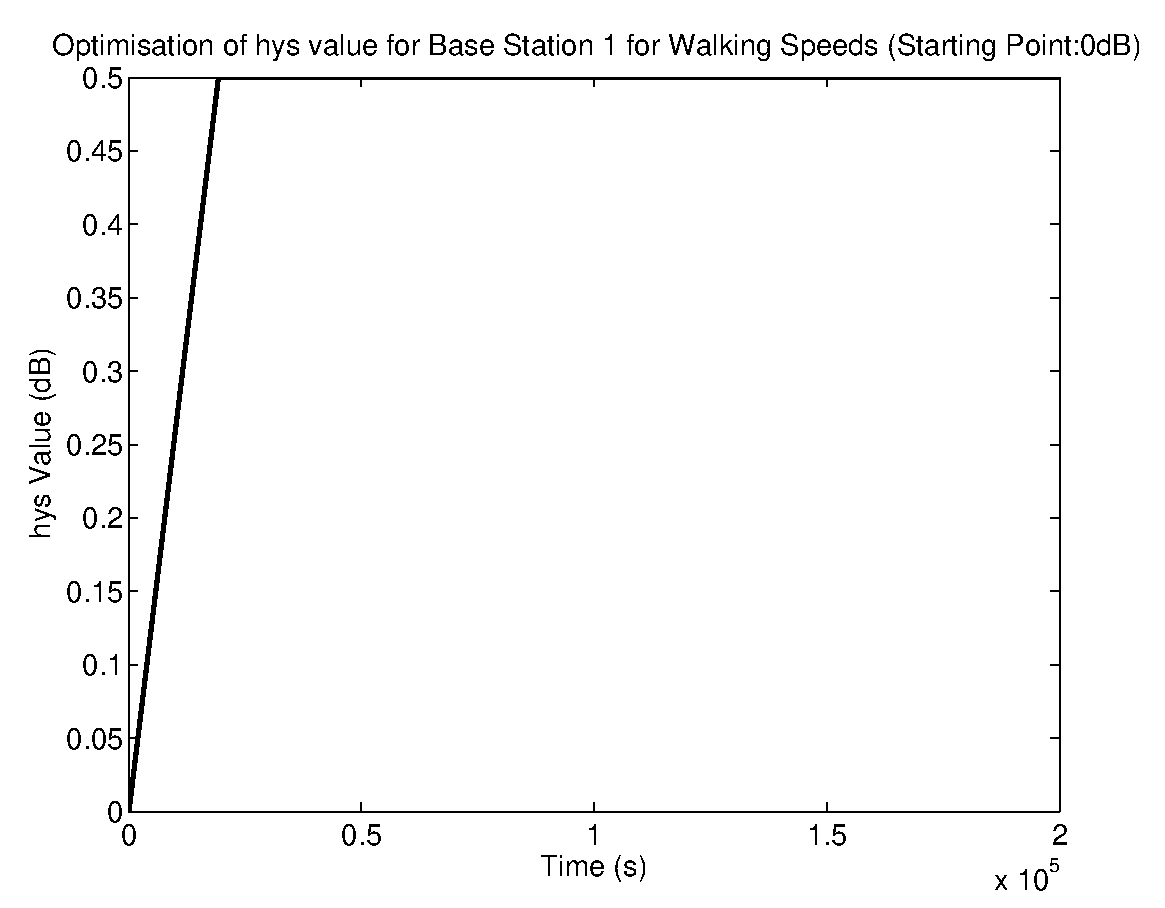
\includegraphics[width=\textwidth]{figures/graphs/walklow/hys1.eps}
                \caption{Changing hys Values}
        \end{subfigure}
        \caption{Illustration of how the TTT and hys values change for Base Station 1 starting at TTT=0s and hys=0dB with UEs moving at walking speeds.}
\end{figure}
\begin{figure}[H]
        \centering
        \begin{subfigure}[b]{0.49\textwidth}
                \includegraphics[width=\textwidth]{figures/graphs/walklow/TTT2.eps}
                \caption{Changing TTT Values}
        \end{subfigure}%
        ~ %add desired spacing between images, e. g. ~, \quad, \qquad etc.
          %(or a blank line to force the subfigure onto a new line)
        \begin{subfigure}[b]{0.49\textwidth}
                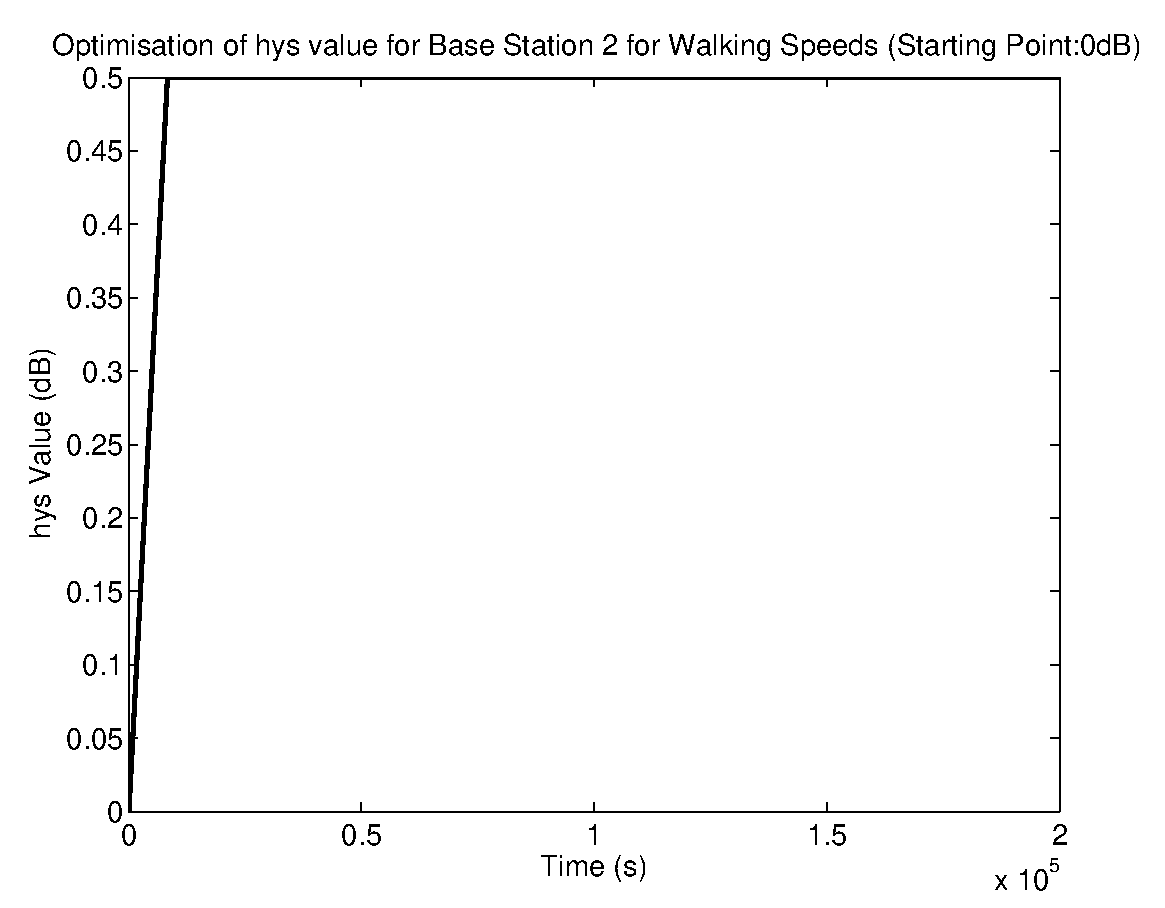
\includegraphics[width=\textwidth]{figures/graphs/walklow/hys2.eps}
                \caption{Changing hys Values}
        \end{subfigure}
        \caption{Illustration of how the TTT and hys values change for Base Station 2 starting at TTT=0s and hys=0dB with UEs moving at walking speeds.}
\end{figure}
\begin{figure}[H]
        \centering
        \begin{subfigure}[b]{0.49\textwidth}
                \includegraphics[width=\textwidth]{figures/graphs/walklow/TTT3.eps}
                \caption{Changing TTT Values}
        \end{subfigure}%
        ~ %add desired spacing between images, e. g. ~, \quad, \qquad etc.
          %(or a blank line to force the subfigure onto a new line)
        \begin{subfigure}[b]{0.49\textwidth}
                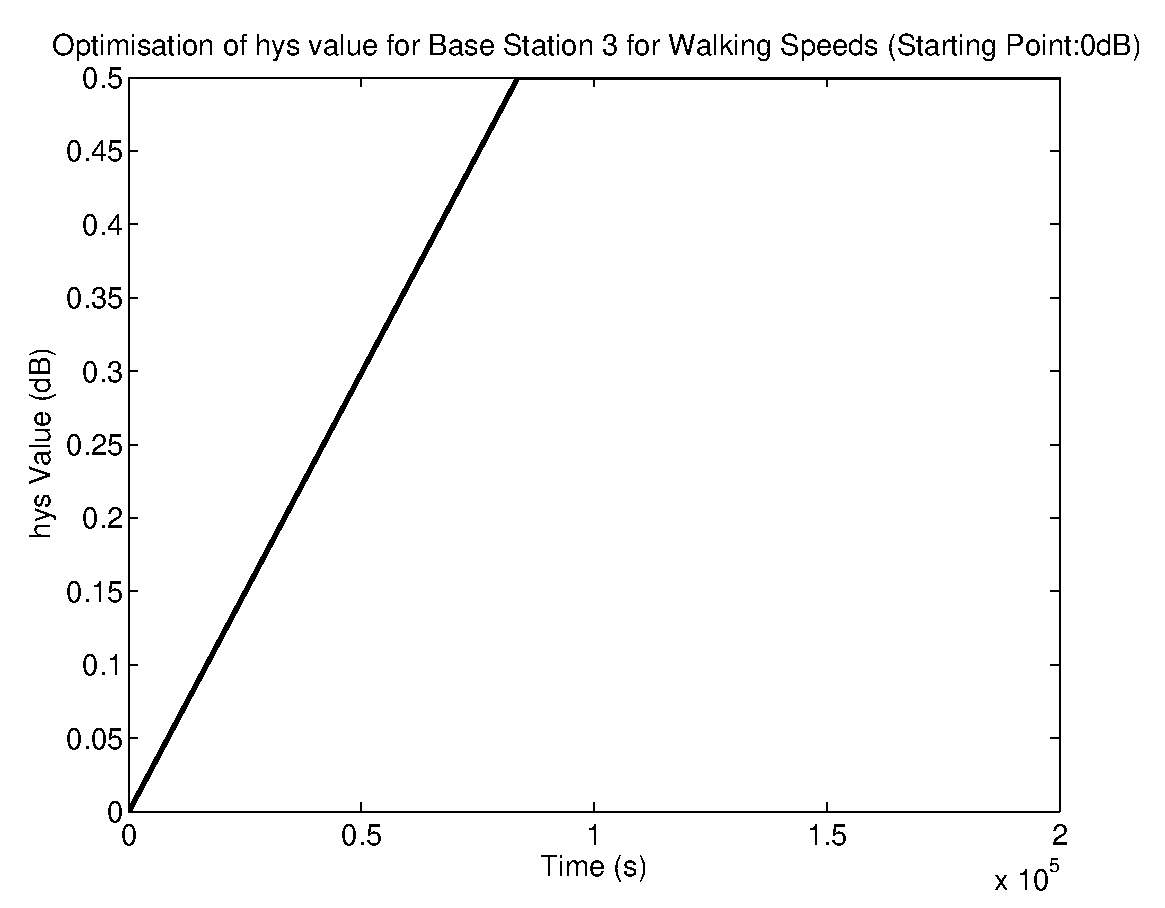
\includegraphics[width=\textwidth]{figures/graphs/walklow/hys3.eps}
                \caption{Changing hys Values}
        \end{subfigure}
        \caption{Illustration of how the TTT and hys values change for Base Station 3 starting at TTT=0s and hys=0dB with UEs moving at walking speeds.}
\end{figure}
\begin{figure}[H]
        \centering
        \begin{subfigure}[b]{0.49\textwidth}
                \includegraphics[width=\textwidth]{figures/graphs/walklow/TTT4.eps}
                \caption{Changing TTT Values}
        \end{subfigure}%
        ~ %add desired spacing between images, e. g. ~, \quad, \qquad etc.
          %(or a blank line to force the subfigure onto a new line)
        \begin{subfigure}[b]{0.49\textwidth}
                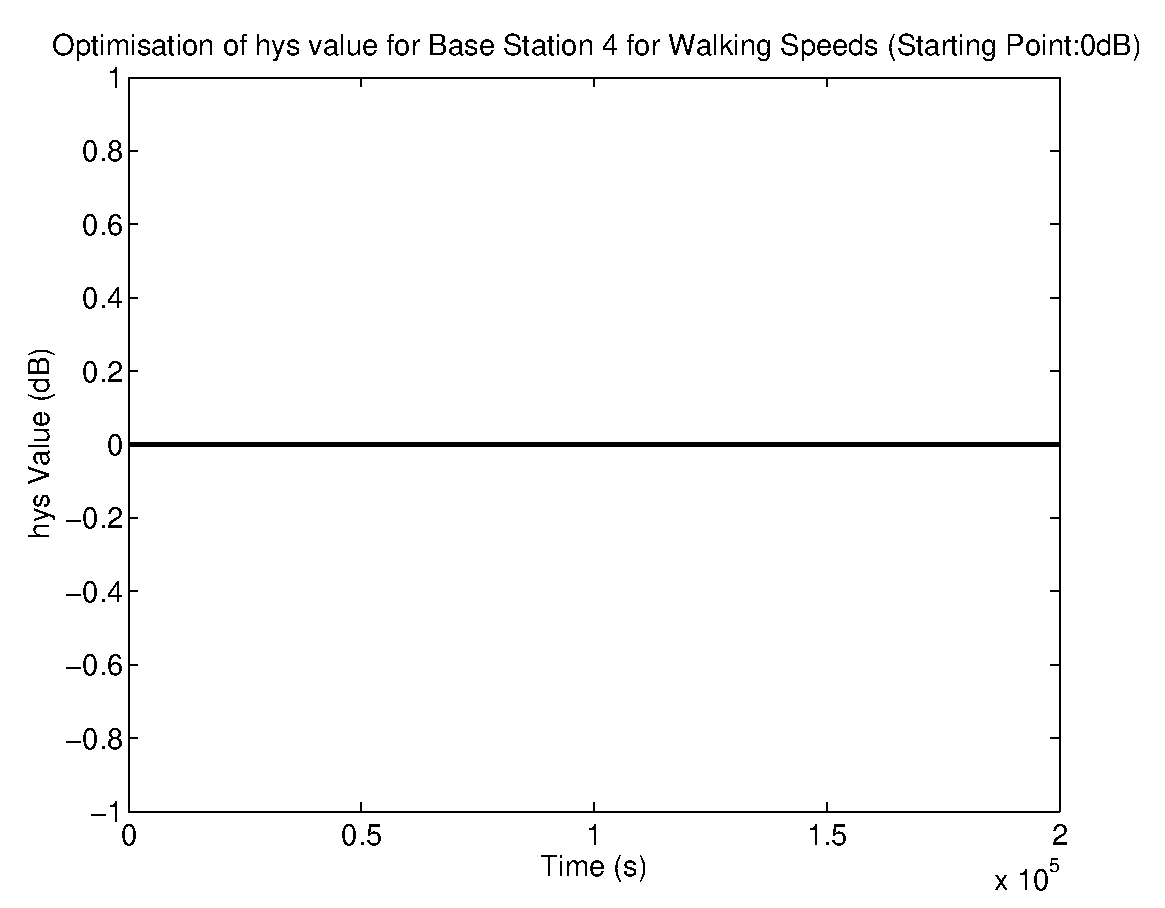
\includegraphics[width=\textwidth]{figures/graphs/walklow/hys4.eps}
                \caption{Changing hys Values}
        \end{subfigure}
        \caption{Illustration of how the TTT and hys values change for Base Station 4 starting at TTT=0s and hys=0dB with UEs moving at walking speeds.}
\end{figure}
\begin{figure}[H]
        \centering
        \begin{subfigure}[b]{0.49\textwidth}
                \includegraphics[width=\textwidth]{figures/graphs/walklow/TTT5.eps}
                \caption{Changing TTT Values}
        \end{subfigure}%
        ~ %add desired spacing between images, e. g. ~, \quad, \qquad etc.
          %(or a blank line to force the subfigure onto a new line)
        \begin{subfigure}[b]{0.49\textwidth}
                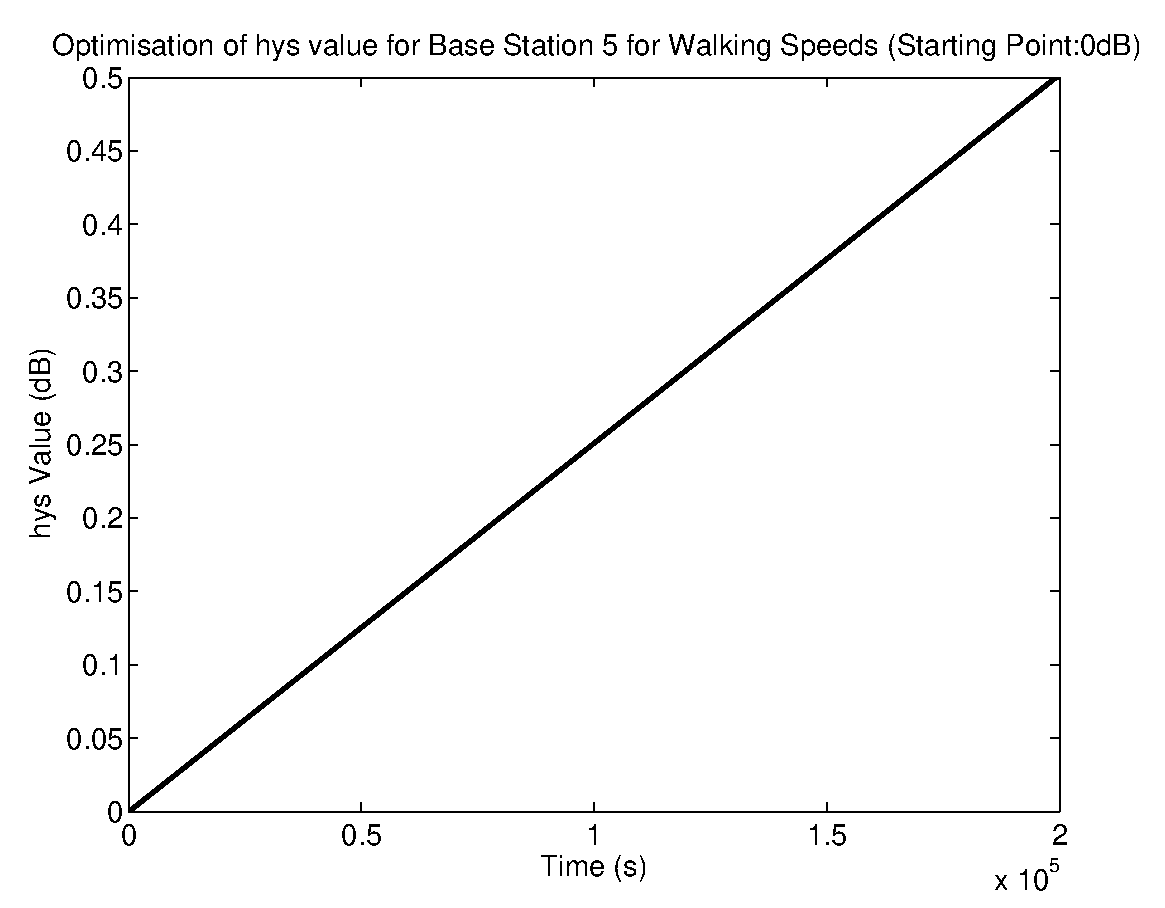
\includegraphics[width=\textwidth]{figures/graphs/walklow/hys5.eps}
                \caption{Changing hys Values}
        \end{subfigure}
        \caption{Illustration of how the TTT and hys values change for Base Station 5 starting at TTT=0s and hys=0dB with UEs moving at walking speeds.}
\end{figure}
\begin{figure}[H]
        \centering
        \begin{subfigure}[b]{0.49\textwidth}
                \includegraphics[width=\textwidth]{figures/graphs/walklow/TTT6.eps}
                \caption{Changing TTT Values}
        \end{subfigure}%
        ~ %add desired spacing between images, e. g. ~, \quad, \qquad etc.
          %(or a blank line to force the subfigure onto a new line)
        \begin{subfigure}[b]{0.49\textwidth}
                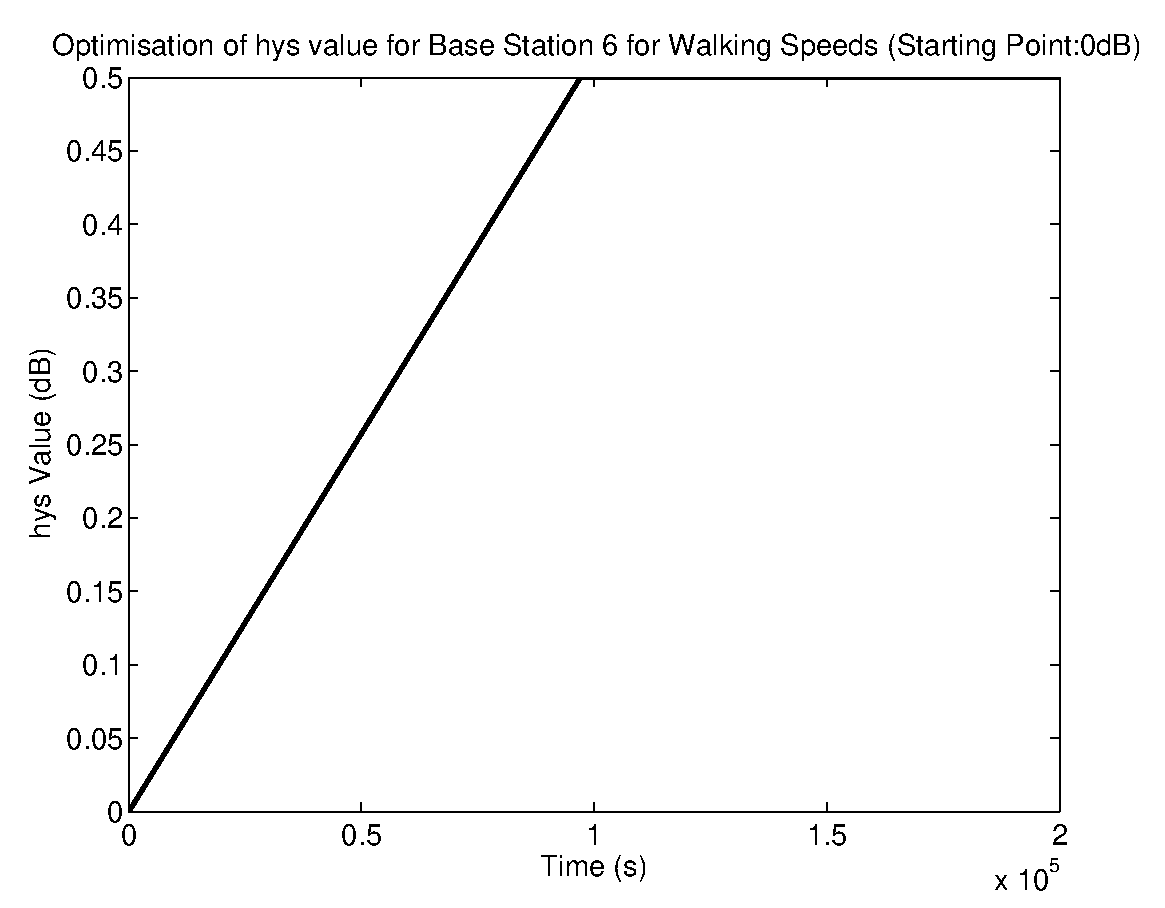
\includegraphics[width=\textwidth]{figures/graphs/walklow/hys6.eps}
                \caption{Changing hys Values}
        \end{subfigure}
        \caption{Illustration of how the TTT and hys values change for Base Station 6 starting at TTT=0s and hys=0dB with UEs moving at walking speeds.}
\end{figure}
\begin{figure}[H]
        \centering
        \begin{subfigure}[b]{0.49\textwidth}
                \includegraphics[width=\textwidth]{figures/graphs/walklow/TTT7.eps}
                \caption{Changing TTT Values}
        \end{subfigure}%
        ~ %add desired spacing between images, e. g. ~, \quad, \qquad etc.
          %(or a blank line to force the subfigure onto a new line)
        \begin{subfigure}[b]{0.49\textwidth}
                \includegraphics[width=\textwidth]{figures/graphs/walklow/hys7.eps}
                \caption{Changing hys Values}
        \end{subfigure}
        \caption{Illustration of how the TTT and hys values change for Base Station 7 starting at TTT=0s and hys=0dB with UEs moving at walking speeds.}
\end{figure}
\begin{figure}[H]
        \centering
        \begin{subfigure}[b]{0.49\textwidth}
                \includegraphics[width=\textwidth]{figures/graphs/walklow/TTT8.eps}
                \caption{Changing TTT Values}
        \end{subfigure}%
        ~ %add desired spacing between images, e. g. ~, \quad, \qquad etc.
          %(or a blank line to force the subfigure onto a new line)
        \begin{subfigure}[b]{0.49\textwidth}
                \includegraphics[width=\textwidth]{figures/graphs/walklow/hys8.eps}
                \caption{Changing hys Values}
        \end{subfigure}
        \caption{Illustration of how the TTT and hys values change for Base Station 8 starting at TTT=0s and hys=0dB with UEs moving at walking speeds.}
\end{figure}
\subsection{Large hys and Small TTT Starting Values}\label{ap:walk_highhys}
\begin{figure}[H]
        \centering
        \begin{subfigure}[b]{0.49\textwidth}
                \includegraphics[width=\textwidth]{figures/graphs/walkhighhys/TTT0.eps}
                \caption{Changing TTT Values}
        \end{subfigure}%
        ~ %add desired spacing between images, e. g. ~, \quad, \qquad etc.
          %(or a blank line to force the subfigure onto a new line)
        \begin{subfigure}[b]{0.49\textwidth}
                \includegraphics[width=\textwidth]{figures/graphs/walkhighhys/hys0.eps}
                \caption{Changing hys Values}
        \end{subfigure}
        \caption{Illustration of how the TTT and hys values change for Base Station 0 starting at TTT=0.08s and hys=7.5dB with UEs moving at walking speeds.}
\end{figure}
\begin{figure}[H]
        \centering
        \begin{subfigure}[b]{0.49\textwidth}
                \includegraphics[width=\textwidth]{figures/graphs/walkhighhys/TTT1.eps}
                \caption{Changing TTT Values}
        \end{subfigure}%
        ~ %add desired spacing between images, e. g. ~, \quad, \qquad etc.
          %(or a blank line to force the subfigure onto a new line)
        \begin{subfigure}[b]{0.49\textwidth}
                \includegraphics[width=\textwidth]{figures/graphs/walkhighhys/hys1.eps}
                \caption{Changing hys Values}
        \end{subfigure}
        \caption{Illustration of how the TTT and hys values change for Base Station 1 starting at TTT=0.08s and hys=7.5dB with UEs moving at walking speeds.}
\end{figure}
\begin{figure}[H]
        \centering
        \begin{subfigure}[b]{0.49\textwidth}
                \includegraphics[width=\textwidth]{figures/graphs/walkhighhys/TTT2.eps}
                \caption{Changing TTT Values}
        \end{subfigure}%
        ~ %add desired spacing between images, e. g. ~, \quad, \qquad etc.
          %(or a blank line to force the subfigure onto a new line)
        \begin{subfigure}[b]{0.49\textwidth}
                \includegraphics[width=\textwidth]{figures/graphs/walkhighhys/hys2.eps}
                \caption{Changing hys Values}
        \end{subfigure}
        \caption{Illustration of how the TTT and hys values change for Base Station 2 starting at TTT=0.08s and hys=7.5dB with UEs moving at walking speeds.}
\end{figure}
\begin{figure}[H]
        \centering
        \begin{subfigure}[b]{0.49\textwidth}
                \includegraphics[width=\textwidth]{figures/graphs/walkhighhys/TTT3.eps}
                \caption{Changing TTT Values}
        \end{subfigure}%
        ~ %add desired spacing between images, e. g. ~, \quad, \qquad etc.
          %(or a blank line to force the subfigure onto a new line)
        \begin{subfigure}[b]{0.49\textwidth}
                \includegraphics[width=\textwidth]{figures/graphs/walkhighhys/hys3.eps}
                \caption{Changing hys Values}
        \end{subfigure}
        \caption{Illustration of how the TTT and hys values change for Base Station 3 starting at TTT=0.08s and hys=7.5dB with UEs moving at walking speeds.}
\end{figure}
\begin{figure}[H]
        \centering
        \begin{subfigure}[b]{0.49\textwidth}
                \includegraphics[width=\textwidth]{figures/graphs/walkhighhys/TTT4.eps}
                \caption{Changing TTT Values}
        \end{subfigure}%
        ~ %add desired spacing between images, e. g. ~, \quad, \qquad etc.
          %(or a blank line to force the subfigure onto a new line)
        \begin{subfigure}[b]{0.49\textwidth}
                \includegraphics[width=\textwidth]{figures/graphs/walkhighhys/hys4.eps}
                \caption{Changing hys Values}
        \end{subfigure}
        \caption{Illustration of how the TTT and hys values change for Base Station 4 starting at TTT=0.08s and hys=7.5dB with UEs moving at walking speeds.}
\end{figure}
\begin{figure}[H]
        \centering
        \begin{subfigure}[b]{0.49\textwidth}
                \includegraphics[width=\textwidth]{figures/graphs/walkhighhys/TTT5.eps}
                \caption{Changing TTT Values}
        \end{subfigure}%
        ~ %add desired spacing between images, e. g. ~, \quad, \qquad etc.
          %(or a blank line to force the subfigure onto a new line)
        \begin{subfigure}[b]{0.49\textwidth}
                \includegraphics[width=\textwidth]{figures/graphs/walkhighhys/hys5.eps}
                \caption{Changing hys Values}
        \end{subfigure}
        \caption{Illustration of how the TTT and hys values change for Base Station 5 starting at TTT=0.08s and hys=7.5dB with UEs moving at walking speeds.}
\end{figure}
\begin{figure}[H]
        \centering
        \begin{subfigure}[b]{0.49\textwidth}
                \includegraphics[width=\textwidth]{figures/graphs/walkhighhys/TTT6.eps}
                \caption{Changing TTT Values}
        \end{subfigure}%
        ~ %add desired spacing between images, e. g. ~, \quad, \qquad etc.
          %(or a blank line to force the subfigure onto a new line)
        \begin{subfigure}[b]{0.49\textwidth}
                \includegraphics[width=\textwidth]{figures/graphs/walkhighhys/hys6.eps}
                \caption{Changing hys Values}
        \end{subfigure}
        \caption{Illustration of how the TTT and hys values change for Base Station 6 starting at TTT=0.08s and hys=7.5dB with UEs moving at walking speeds.}
\end{figure}
\begin{figure}[H]
        \centering
        \begin{subfigure}[b]{0.49\textwidth}
                \includegraphics[width=\textwidth]{figures/graphs/walkhighhys/TTT7.eps}
                \caption{Changing TTT Values}
        \end{subfigure}%
        ~ %add desired spacing between images, e. g. ~, \quad, \qquad etc.
          %(or a blank line to force the subfigure onto a new line)
        \begin{subfigure}[b]{0.49\textwidth}
                \includegraphics[width=\textwidth]{figures/graphs/walkhighhys/hys7.eps}
                \caption{Changing hys Values}
        \end{subfigure}
        \caption{Illustration of how the TTT and hys values change for Base Station 7 starting at TTT=0.08s and hys=7.5dB with UEs moving at walking speeds.}
\end{figure}
\begin{figure}[H]
        \centering
        \begin{subfigure}[b]{0.49\textwidth}
                \includegraphics[width=\textwidth]{figures/graphs/walkhighhys/TTT8.eps}
                \caption{Changing TTT Values}
        \end{subfigure}%
        ~ %add desired spacing between images, e. g. ~, \quad, \qquad etc.
          %(or a blank line to force the subfigure onto a new line)
        \begin{subfigure}[b]{0.49\textwidth}
                \includegraphics[width=\textwidth]{figures/graphs/walkhighhys/hys8.eps}
                \caption{Changing hys Values}
        \end{subfigure}
        \caption{Illustration of how the TTT and hys values change for Base Station 8 starting at TTT=0.08s and hys=7.5dB with UEs moving at walking speeds.}
\end{figure}
\section{Vehicle Speeds}\label{ap:veh}
\subsection{Large Starting Values}\label{ap:veh_large}
\begin{figure}[H]
        \centering
        \begin{subfigure}[b]{0.49\textwidth}
                \includegraphics[width=\textwidth]{figures/graphs/vehhigh/TTT0.eps}
                \caption{Changing TTT Values}
        \end{subfigure}%
        ~ %add desired spacing between images, e. g. ~, \quad, \qquad etc.
          %(or a blank line to force the subfigure onto a new line)
        \begin{subfigure}[b]{0.49\textwidth}
                \includegraphics[width=\textwidth]{figures/graphs/vehhigh/hys0.eps}
                \caption{Changing hys Values}
        \end{subfigure}
        \caption{Illustration of how the TTT and hys values change for Base Station 0 starting at TTT=5.12s and hys=10dB with UEs moving at vehicle speeds.}
\end{figure}
\begin{figure}[H]
        \centering
        \begin{subfigure}[b]{0.49\textwidth}
                \includegraphics[width=\textwidth]{figures/graphs/vehhigh/TTT1.eps}
                \caption{Changing TTT Values}
        \end{subfigure}%
        ~ %add desired spacing between images, e. g. ~, \quad, \qquad etc.
          %(or a blank line to force the subfigure onto a new line)
        \begin{subfigure}[b]{0.49\textwidth}
                \includegraphics[width=\textwidth]{figures/graphs/vehhigh/hys1.eps}
                \caption{Changing hys Values}
        \end{subfigure}
        \caption{Illustration of how the TTT and hys values change for Base Station 1 starting at TTT=5.12s and hys=10dB with UEs moving at vehicle speeds.}
\end{figure}
\begin{figure}[H]
        \centering
        \begin{subfigure}[b]{0.49\textwidth}
                \includegraphics[width=\textwidth]{figures/graphs/vehhigh/TTT2.eps}
                \caption{Changing TTT Values}
        \end{subfigure}%
        ~ %add desired spacing between images, e. g. ~, \quad, \qquad etc.
          %(or a blank line to force the subfigure onto a new line)
        \begin{subfigure}[b]{0.49\textwidth}
                \includegraphics[width=\textwidth]{figures/graphs/vehhigh/hys2.eps}
                \caption{Changing hys Values}
        \end{subfigure}
        \caption{Illustration of how the TTT and hys values change for Base Station 2 starting at TTT=5.12s and hys=10dB with UEs moving at vehicle speeds.}
\end{figure}
\begin{figure}[H]
        \centering
        \begin{subfigure}[b]{0.49\textwidth}
                \includegraphics[width=\textwidth]{figures/graphs/vehhigh/TTT3.eps}
                \caption{Changing TTT Values}
        \end{subfigure}%
        ~ %add desired spacing between images, e. g. ~, \quad, \qquad etc.
          %(or a blank line to force the subfigure onto a new line)
        \begin{subfigure}[b]{0.49\textwidth}
                \includegraphics[width=\textwidth]{figures/graphs/vehhigh/hys3.eps}
                \caption{Changing hys Values}
        \end{subfigure}
        \caption{Illustration of how the TTT and hys values change for Base Station 3 starting at TTT=5.12s and hys=10dB with UEs moving at vehicle speeds.}
\end{figure}
\begin{figure}[H]
        \centering
        \begin{subfigure}[b]{0.49\textwidth}
                \includegraphics[width=\textwidth]{figures/graphs/vehhigh/TTT4.eps}
                \caption{Changing TTT Values}
        \end{subfigure}%
        ~ %add desired spacing between images, e. g. ~, \quad, \qquad etc.
          %(or a blank line to force the subfigure onto a new line)
        \begin{subfigure}[b]{0.49\textwidth}
                \includegraphics[width=\textwidth]{figures/graphs/vehhigh/hys4.eps}
                \caption{Changing hys Values}
        \end{subfigure}
        \caption{Illustration of how the TTT and hys values change for Base Station 4 starting at TTT=5.12s and hys=10dB with UEs moving at vehicle speeds.}
\end{figure}
\begin{figure}[H]
        \centering
        \begin{subfigure}[b]{0.49\textwidth}
                \includegraphics[width=\textwidth]{figures/graphs/vehhigh/TTT5.eps}
                \caption{Changing TTT Values}
        \end{subfigure}%
        ~ %add desired spacing between images, e. g. ~, \quad, \qquad etc.
          %(or a blank line to force the subfigure onto a new line)
        \begin{subfigure}[b]{0.49\textwidth}
                \includegraphics[width=\textwidth]{figures/graphs/vehhigh/hys5.eps}
                \caption{Changing hys Values}
        \end{subfigure}
        \caption{Illustration of how the TTT and hys values change for Base Station 5 starting at TTT=5.12s and hys=10dB with UEs moving at vehicle speeds.}
\end{figure}
\begin{figure}[H]
        \centering
        \begin{subfigure}[b]{0.49\textwidth}
                \includegraphics[width=\textwidth]{figures/graphs/vehhigh/TTT6.eps}
                \caption{Changing TTT Values}
        \end{subfigure}%
        ~ %add desired spacing between images, e. g. ~, \quad, \qquad etc.
          %(or a blank line to force the subfigure onto a new line)
        \begin{subfigure}[b]{0.49\textwidth}
                \includegraphics[width=\textwidth]{figures/graphs/vehhigh/hys6.eps}
                \caption{Changing hys Values}
        \end{subfigure}
        \caption{Illustration of how the TTT and hys values change for Base Station 6 starting at TTT=5.12s and hys=10dB with UEs moving at vehicle speeds.}
\end{figure}
\begin{figure}[H]
        \centering
        \begin{subfigure}[b]{0.49\textwidth}
                \includegraphics[width=\textwidth]{figures/graphs/vehhigh/TTT7.eps}
                \caption{Changing TTT Values}
        \end{subfigure}%
        ~ %add desired spacing between images, e. g. ~, \quad, \qquad etc.
          %(or a blank line to force the subfigure onto a new line)
        \begin{subfigure}[b]{0.49\textwidth}
                \includegraphics[width=\textwidth]{figures/graphs/vehhigh/hys7.eps}
                \caption{Changing hys Values}
        \end{subfigure}
        \caption{Illustration of how the TTT and hys values change for Base Station 7 starting at TTT=5.12s and hys=10dB with UEs moving at vehicle speeds.}
\end{figure}
\begin{figure}[H]
        \centering
        \begin{subfigure}[b]{0.49\textwidth}
                \includegraphics[width=\textwidth]{figures/graphs/vehhigh/TTT8.eps}
                \caption{Changing TTT Values}
        \end{subfigure}%
        ~ %add desired spacing between images, e. g. ~, \quad, \qquad etc.
          %(or a blank line to force the subfigure onto a new line)
        \begin{subfigure}[b]{0.49\textwidth}
                \includegraphics[width=\textwidth]{figures/graphs/vehhigh/hys8.eps}
                \caption{Changing hys Values}
        \end{subfigure}
        \caption{Illustration of how the TTT and hys values change for Base Station 8 starting at TTT=5.12s and hys=10dB with UEs moving at vehicle speeds.}
\end{figure}
\subsection{Middle Starting Values}\label{ap:veh_mid}
\begin{figure}[H]
        \centering
        \begin{subfigure}[b]{0.49\textwidth}
                \includegraphics[width=\textwidth]{figures/graphs/vehmid/TTT0.eps}
                \caption{Changing TTT Values}
        \end{subfigure}%
        ~ %add desired spacing between images, e. g. ~, \quad, \qquad etc.
          %(or a blank line to force the subfigure onto a new line)
        \begin{subfigure}[b]{0.49\textwidth}
                \includegraphics[width=\textwidth]{figures/graphs/vehmid/hys0.eps}
                \caption{Changing hys Values}
        \end{subfigure}
        \caption{Illustration of how the TTT and hys values change for Base Station 0 starting at TTT=0.256s and hys=5dB with UEs moving at vehicle speeds.}
\end{figure}
\begin{figure}[H]
        \centering
        \begin{subfigure}[b]{0.49\textwidth}
                \includegraphics[width=\textwidth]{figures/graphs/vehmid/TTT1.eps}
                \caption{Changing TTT Values}
        \end{subfigure}%
        ~ %add desired spacing between images, e. g. ~, \quad, \qquad etc.
          %(or a blank line to force the subfigure onto a new line)
        \begin{subfigure}[b]{0.49\textwidth}
                \includegraphics[width=\textwidth]{figures/graphs/vehmid/hys1.eps}
                \caption{Changing hys Values}
        \end{subfigure}
        \caption{Illustration of how the TTT and hys values change for Base Station 1 starting at TTT=0.256s and hys=5dB with UEs moving at vehicle speeds.}
\end{figure}
\begin{figure}[H]
        \centering
        \begin{subfigure}[b]{0.49\textwidth}
                \includegraphics[width=\textwidth]{figures/graphs/vehmid/TTT2.eps}
                \caption{Changing TTT Values}
        \end{subfigure}%
        ~ %add desired spacing between images, e. g. ~, \quad, \qquad etc.
          %(or a blank line to force the subfigure onto a new line)
        \begin{subfigure}[b]{0.49\textwidth}
                \includegraphics[width=\textwidth]{figures/graphs/vehmid/hys2.eps}
                \caption{Changing hys Values}
        \end{subfigure}
        \caption{Illustration of how the TTT and hys values change for Base Station 2 starting at TTT=0.256s and hys=5dB with UEs moving at vehicle speeds.}
\end{figure}
\begin{figure}[H]
        \centering
        \begin{subfigure}[b]{0.49\textwidth}
                \includegraphics[width=\textwidth]{figures/graphs/vehmid/TTT3.eps}
                \caption{Changing TTT Values}
        \end{subfigure}%
        ~ %add desired spacing between images, e. g. ~, \quad, \qquad etc.
          %(or a blank line to force the subfigure onto a new line)
        \begin{subfigure}[b]{0.49\textwidth}
                \includegraphics[width=\textwidth]{figures/graphs/vehmid/hys3.eps}
                \caption{Changing hys Values}
        \end{subfigure}
        \caption{Illustration of how the TTT and hys values change for Base Station 3 starting at TTT=0.256s and hys=5dB with UEs moving at vehicle speeds.}
\end{figure}
\begin{figure}[H]
        \centering
        \begin{subfigure}[b]{0.49\textwidth}
                \includegraphics[width=\textwidth]{figures/graphs/vehmid/TTT4.eps}
                \caption{Changing TTT Values}
        \end{subfigure}%
        ~ %add desired spacing between images, e. g. ~, \quad, \qquad etc.
          %(or a blank line to force the subfigure onto a new line)
        \begin{subfigure}[b]{0.49\textwidth}
                \includegraphics[width=\textwidth]{figures/graphs/vehmid/hys4.eps}
                \caption{Changing hys Values}
        \end{subfigure}
        \caption{Illustration of how the TTT and hys values change for Base Station 4 starting at TTT=0.256s and hys=5dB with UEs moving at vehicle speeds.}
\end{figure}
\begin{figure}[H]
        \centering
        \begin{subfigure}[b]{0.49\textwidth}
                \includegraphics[width=\textwidth]{figures/graphs/vehmid/TTT5.eps}
                \caption{Changing TTT Values}
        \end{subfigure}%
        ~ %add desired spacing between images, e. g. ~, \quad, \qquad etc.
          %(or a blank line to force the subfigure onto a new line)
        \begin{subfigure}[b]{0.49\textwidth}
                \includegraphics[width=\textwidth]{figures/graphs/vehmid/hys5.eps}
                \caption{Changing hys Values}
        \end{subfigure}
        \caption{Illustration of how the TTT and hys values change for Base Station 5 starting at TTT=0.256s and hys=5dB with UEs moving at vehicle speeds.}
\end{figure}
\begin{figure}[H]
        \centering
        \begin{subfigure}[b]{0.49\textwidth}
                \includegraphics[width=\textwidth]{figures/graphs/vehmid/TTT6.eps}
                \caption{Changing TTT Values}
        \end{subfigure}%
        ~ %add desired spacing between images, e. g. ~, \quad, \qquad etc.
          %(or a blank line to force the subfigure onto a new line)
        \begin{subfigure}[b]{0.49\textwidth}
                \includegraphics[width=\textwidth]{figures/graphs/vehmid/hys6.eps}
                \caption{Changing hys Values}
        \end{subfigure}
        \caption{Illustration of how the TTT and hys values change for Base Station 6 starting at TTT=0.256s and hys=5dB with UEs moving at vehicle speeds.}
\end{figure}
\begin{figure}[H]
        \centering
        \begin{subfigure}[b]{0.49\textwidth}
                \includegraphics[width=\textwidth]{figures/graphs/vehmid/TTT7.eps}
                \caption{Changing TTT Values}
        \end{subfigure}%
        ~ %add desired spacing between images, e. g. ~, \quad, \qquad etc.
          %(or a blank line to force the subfigure onto a new line)
        \begin{subfigure}[b]{0.49\textwidth}
                \includegraphics[width=\textwidth]{figures/graphs/vehmid/hys7.eps}
                \caption{Changing hys Values}
        \end{subfigure}
        \caption{Illustration of how the TTT and hys values change for Base Station 7 starting at TTT=0.256s and hys=5dB with UEs moving at vehicle speeds.}
\end{figure}
\begin{figure}[H]
        \centering
        \begin{subfigure}[b]{0.49\textwidth}
                \includegraphics[width=\textwidth]{figures/graphs/vehmid/TTT8.eps}
                \caption{Changing TTT Values}
        \end{subfigure}%
        ~ %add desired spacing between images, e. g. ~, \quad, \qquad etc.
          %(or a blank line to force the subfigure onto a new line)
        \begin{subfigure}[b]{0.49\textwidth}
                \includegraphics[width=\textwidth]{figures/graphs/vehmid/hys8.eps}
                \caption{Changing hys Values}
        \end{subfigure}
        \caption{Illustration of how the TTT and hys values change for Base Station 8 starting at TTT=0.256s and hys=5dB with UEs moving at vehicle speeds.}
\end{figure}
\subsection{Small Starting Values}\label{ap:veh_low}
\begin{figure}[H]
        \centering
        \begin{subfigure}[b]{0.49\textwidth}
                \includegraphics[width=\textwidth]{figures/graphs/vehlow/TTT0.eps}
                \caption{Changing TTT Values}
        \end{subfigure}%
        ~ %add desired spacing between images, e. g. ~, \quad, \qquad etc.
          %(or a blank line to force the subfigure onto a new line)
        \begin{subfigure}[b]{0.49\textwidth}
                \includegraphics[width=\textwidth]{figures/graphs/vehlow/hys0.eps}
                \caption{Changing hys Values}
        \end{subfigure}
        \caption{Illustration of how the TTT and hys values change for Base Station 0 starting at TTT=0s and hys=0dB with UEs moving at vehicle speeds.}
\end{figure}
\begin{figure}[H]
        \centering
        \begin{subfigure}[b]{0.49\textwidth}
                \includegraphics[width=\textwidth]{figures/graphs/vehlow/TTT1.eps}
                \caption{Changing TTT Values}
        \end{subfigure}%
        ~ %add desired spacing between images, e. g. ~, \quad, \qquad etc.
          %(or a blank line to force the subfigure onto a new line)
        \begin{subfigure}[b]{0.49\textwidth}
                \includegraphics[width=\textwidth]{figures/graphs/vehlow/hys1.eps}
                \caption{Changing hys Values}
        \end{subfigure}
        \caption{Illustration of how the TTT and hys values change for Base Station 1 starting at TTT=0s and hys=0dB with UEs moving at vehicle speeds.}
\end{figure}
\begin{figure}[H]
        \centering
        \begin{subfigure}[b]{0.49\textwidth}
                \includegraphics[width=\textwidth]{figures/graphs/vehlow/TTT2.eps}
                \caption{Changing TTT Values}
        \end{subfigure}%
        ~ %add desired spacing between images, e. g. ~, \quad, \qquad etc.
          %(or a blank line to force the subfigure onto a new line)
        \begin{subfigure}[b]{0.49\textwidth}
                \includegraphics[width=\textwidth]{figures/graphs/vehlow/hys2.eps}
                \caption{Changing hys Values}
        \end{subfigure}
        \caption{Illustration of how the TTT and hys values change for Base Station 2 starting at TTT=0s and hys=0dB with UEs moving at vehicle speeds.}
\end{figure}
\begin{figure}[H]
        \centering
        \begin{subfigure}[b]{0.49\textwidth}
                \includegraphics[width=\textwidth]{figures/graphs/vehlow/TTT3.eps}
                \caption{Changing TTT Values}
        \end{subfigure}%
        ~ %add desired spacing between images, e. g. ~, \quad, \qquad etc.
          %(or a blank line to force the subfigure onto a new line)
        \begin{subfigure}[b]{0.49\textwidth}
                \includegraphics[width=\textwidth]{figures/graphs/vehlow/hys3.eps}
                \caption{Changing hys Values}
        \end{subfigure}
        \caption{Illustration of how the TTT and hys values change for Base Station 3 starting at TTT=0s and hys=0dB with UEs moving at vehicle speeds.}
\end{figure}
\begin{figure}[H]
        \centering
        \begin{subfigure}[b]{0.49\textwidth}
                \includegraphics[width=\textwidth]{figures/graphs/vehlow/TTT4.eps}
                \caption{Changing TTT Values}
        \end{subfigure}%
        ~ %add desired spacing between images, e. g. ~, \quad, \qquad etc.
          %(or a blank line to force the subfigure onto a new line)
        \begin{subfigure}[b]{0.49\textwidth}
                \includegraphics[width=\textwidth]{figures/graphs/vehlow/hys4.eps}
                \caption{Changing hys Values}
        \end{subfigure}
        \caption{Illustration of how the TTT and hys values change for Base Station 4 starting at TTT=0s and hys=0dB with UEs moving at vehicle speeds.}
\end{figure}
\begin{figure}[H]
        \centering
        \begin{subfigure}[b]{0.49\textwidth}
                \includegraphics[width=\textwidth]{figures/graphs/vehlow/TTT5.eps}
                \caption{Changing TTT Values}
        \end{subfigure}%
        ~ %add desired spacing between images, e. g. ~, \quad, \qquad etc.
          %(or a blank line to force the subfigure onto a new line)
        \begin{subfigure}[b]{0.49\textwidth}
                \includegraphics[width=\textwidth]{figures/graphs/vehlow/hys5.eps}
                \caption{Changing hys Values}
        \end{subfigure}
        \caption{Illustration of how the TTT and hys values change for Base Station 5 starting at TTT=0s and hys=0dB with UEs moving at vehicle speeds.}
\end{figure}
\begin{figure}[H]
        \centering
        \begin{subfigure}[b]{0.49\textwidth}
                \includegraphics[width=\textwidth]{figures/graphs/vehlow/TTT6.eps}
                \caption{Changing TTT Values}
        \end{subfigure}%
        ~ %add desired spacing between images, e. g. ~, \quad, \qquad etc.
          %(or a blank line to force the subfigure onto a new line)
        \begin{subfigure}[b]{0.49\textwidth}
                \includegraphics[width=\textwidth]{figures/graphs/vehlow/hys6.eps}
                \caption{Changing hys Values}
        \end{subfigure}
        \caption{Illustration of how the TTT and hys values change for Base Station 6 starting at TTT=0s and hys=0dB with UEs moving at vehicle speeds.}
\end{figure}
\begin{figure}[H]
        \centering
        \begin{subfigure}[b]{0.49\textwidth}
                \includegraphics[width=\textwidth]{figures/graphs/vehlow/TTT7.eps}
                \caption{Changing TTT Values}
        \end{subfigure}%
        ~ %add desired spacing between images, e. g. ~, \quad, \qquad etc.
          %(or a blank line to force the subfigure onto a new line)
        \begin{subfigure}[b]{0.49\textwidth}
                \includegraphics[width=\textwidth]{figures/graphs/vehlow/hys7.eps}
                \caption{Changing hys Values}
        \end{subfigure}
        \caption{Illustration of how the TTT and hys values change for Base Station 7 starting at TTT=0s and hys=0dB with UEs moving at vehicle speeds.}
\end{figure}
\begin{figure}[H]
        \centering
        \begin{subfigure}[b]{0.49\textwidth}
                \includegraphics[width=\textwidth]{figures/graphs/vehlow/TTT8.eps}
                \caption{Changing TTT Values}
        \end{subfigure}%
        ~ %add desired spacing between images, e. g. ~, \quad, \qquad etc.
          %(or a blank line to force the subfigure onto a new line)
        \begin{subfigure}[b]{0.49\textwidth}
                \includegraphics[width=\textwidth]{figures/graphs/vehlow/hys8.eps}
                \caption{Changing hys Values}
        \end{subfigure}
        \caption{Illustration of how the TTT and hys values change for Base Station 8 starting at TTT=0s and hys=0dB with UEs moving at vehicle speeds.}
\end{figure}
\subsection{Large hys and Small TTT Starting Values}\label{ap:veh_highhys}
\begin{figure}[H]
        \centering
        \begin{subfigure}[b]{0.49\textwidth}
                \includegraphics[width=\textwidth]{figures/graphs/vehhighhys/TTT0.eps}
                \caption{Changing TTT Values}
        \end{subfigure}%
        ~ %add desired spacing between images, e. g. ~, \quad, \qquad etc.
          %(or a blank line to force the subfigure onto a new line)
        \begin{subfigure}[b]{0.49\textwidth}
                \includegraphics[width=\textwidth]{figures/graphs/vehhighhys/hys0.eps}
                \caption{Changing hys Values}
        \end{subfigure}
        \caption{Illustration of how the TTT and hys values change for Base Station 0 starting at TTT=0.08s and hys=7.5dB with UEs moving at vehicle speeds.}
\end{figure}
\begin{figure}[H]
        \centering
        \begin{subfigure}[b]{0.49\textwidth}
                \includegraphics[width=\textwidth]{figures/graphs/vehhighhys/TTT1.eps}
                \caption{Changing TTT Values}
        \end{subfigure}%
        ~ %add desired spacing between images, e. g. ~, \quad, \qquad etc.
          %(or a blank line to force the subfigure onto a new line)
        \begin{subfigure}[b]{0.49\textwidth}
                \includegraphics[width=\textwidth]{figures/graphs/vehhighhys/hys1.eps}
                \caption{Changing hys Values}
        \end{subfigure}
        \caption{Illustration of how the TTT and hys values change for Base Station 1 starting at TTT=0.08s and hys=7.5dB with UEs moving at vehicle speeds.}
\end{figure}
\begin{figure}[H]
        \centering
        \begin{subfigure}[b]{0.49\textwidth}
                \includegraphics[width=\textwidth]{figures/graphs/vehhighhys/TTT2.eps}
                \caption{Changing TTT Values}
        \end{subfigure}%
        ~ %add desired spacing between images, e. g. ~, \quad, \qquad etc.
          %(or a blank line to force the subfigure onto a new line)
        \begin{subfigure}[b]{0.49\textwidth}
                \includegraphics[width=\textwidth]{figures/graphs/vehhighhys/hys2.eps}
                \caption{Changing hys Values}
        \end{subfigure}
        \caption{Illustration of how the TTT and hys values change for Base Station 2 starting at TTT=0.08s and hys=7.5dB with UEs moving at vehicle speeds.}
\end{figure}
\begin{figure}[H]
        \centering
        \begin{subfigure}[b]{0.49\textwidth}
                \includegraphics[width=\textwidth]{figures/graphs/vehhighhys/TTT3.eps}
                \caption{Changing TTT Values}
        \end{subfigure}%
        ~ %add desired spacing between images, e. g. ~, \quad, \qquad etc.
          %(or a blank line to force the subfigure onto a new line)
        \begin{subfigure}[b]{0.49\textwidth}
                \includegraphics[width=\textwidth]{figures/graphs/vehhighhys/hys3.eps}
                \caption{Changing hys Values}
        \end{subfigure}
        \caption{Illustration of how the TTT and hys values change for Base Station 3 starting at TTT=0.08s and hys=7.5dB with UEs moving at vehicle speeds.}
\end{figure}
\begin{figure}[H]
        \centering
        \begin{subfigure}[b]{0.49\textwidth}
                \includegraphics[width=\textwidth]{figures/graphs/vehhighhys/TTT4.eps}
                \caption{Changing TTT Values}
        \end{subfigure}%
        ~ %add desired spacing between images, e. g. ~, \quad, \qquad etc.
          %(or a blank line to force the subfigure onto a new line)
        \begin{subfigure}[b]{0.49\textwidth}
                \includegraphics[width=\textwidth]{figures/graphs/vehhighhys/hys4.eps}
                \caption{Changing hys Values}
        \end{subfigure}
        \caption{Illustration of how the TTT and hys values change for Base Station 4 starting at TTT=0.08s and hys=7.5dB with UEs moving at vehicle speeds.}
\end{figure}
\begin{figure}[H]
        \centering
        \begin{subfigure}[b]{0.49\textwidth}
                \includegraphics[width=\textwidth]{figures/graphs/vehhighhys/TTT5.eps}
                \caption{Changing TTT Values}
        \end{subfigure}%
        ~ %add desired spacing between images, e. g. ~, \quad, \qquad etc.
          %(or a blank line to force the subfigure onto a new line)
        \begin{subfigure}[b]{0.49\textwidth}
                \includegraphics[width=\textwidth]{figures/graphs/vehhighhys/hys5.eps}
                \caption{Changing hys Values}
        \end{subfigure}
        \caption{Illustration of how the TTT and hys values change for Base Station 5 starting at TTT=0.08s and hys=7.5dB with UEs moving at vehicle speeds.}
\end{figure}
\begin{figure}[H]
        \centering
        \begin{subfigure}[b]{0.49\textwidth}
                \includegraphics[width=\textwidth]{figures/graphs/vehhighhys/TTT6.eps}
                \caption{Changing TTT Values}
        \end{subfigure}%
        ~ %add desired spacing between images, e. g. ~, \quad, \qquad etc.
          %(or a blank line to force the subfigure onto a new line)
        \begin{subfigure}[b]{0.49\textwidth}
                \includegraphics[width=\textwidth]{figures/graphs/vehhighhys/hys6.eps}
                \caption{Changing hys Values}
        \end{subfigure}
        \caption{Illustration of how the TTT and hys values change for Base Station 6 starting at TTT=0.08s and hys=7.5dB with UEs moving at vehicle speeds.}
\end{figure}
\begin{figure}[H]
        \centering
        \begin{subfigure}[b]{0.49\textwidth}
                \includegraphics[width=\textwidth]{figures/graphs/vehhighhys/TTT7.eps}
                \caption{Changing TTT Values}
        \end{subfigure}%
        ~ %add desired spacing between images, e. g. ~, \quad, \qquad etc.
          %(or a blank line to force the subfigure onto a new line)
        \begin{subfigure}[b]{0.49\textwidth}
                \includegraphics[width=\textwidth]{figures/graphs/vehhighhys/hys7.eps}
                \caption{Changing hys Values}
        \end{subfigure}
        \caption{Illustration of how the TTT and hys values change for Base Station 7 starting at TTT=0.08s and hys=7.5dB with UEs moving at vehicle speeds.}
\end{figure}
\begin{figure}[H]
        \centering
        \begin{subfigure}[b]{0.49\textwidth}
                \includegraphics[width=\textwidth]{figures/graphs/vehhighhys/TTT8.eps}
                \caption{Changing TTT Values}
        \end{subfigure}%
        ~ %add desired spacing between images, e. g. ~, \quad, \qquad etc.
          %(or a blank line to force the subfigure onto a new line)
        \begin{subfigure}[b]{0.49\textwidth}
                \includegraphics[width=\textwidth]{figures/graphs/vehhighhys/hys8.eps}
                \caption{Changing hys Values}
        \end{subfigure}
        \caption{Illustration of how the TTT and hys values change for Base Station 8 starting at TTT=0.08s and hys=7.5dB with UEs moving at vehicle speeds.}
\end{figure}